% !TEX program = pdflatex
% Standalone first draft: compile with
%   latexmk -pdf forced_navier_stokes_blowup.tex
% or
%   pdflatex forced_navier_stokes_blowup.tex && bibtex forced_navier_stokes_blowup && pdflatex forced_navier_stokes_blowup.tex && pdflatex forced_navier_stokes_blowup.tex
%
\begin{filecontents*}{forced_navier_stokes_blowup.bib}
@article{leray1934,
  author  = {Leray, Jean},
  title   = {Sur le mouvement d'un liquide visqueux emplissant l'espace},
  journal = {Acta Mathematica},
  volume  = {63},
  pages   = {193--248},
  year    = {1934}
}

@article{hopf1951,
  author  = {Hopf, Eberhard},
  title   = {{\"U}ber die Anfangswertaufgabe f{\"u}r die hydrodynamischen Grundgleichungen},
  journal = {Mathematische Nachrichten},
  volume  = {4},
  pages   = {213--231},
  year    = {1951}
}

@article{ckn1982,
  author  = {Caffarelli, Luis and Kohn, Robert and Nirenberg, Louis},
  title   = {Partial regularity of suitable weak solutions of the {N}avier--{S}tokes equations},
  journal = {Communications on Pure and Applied Mathematics},
  volume  = {35},
  number  = {6},
  pages   = {771--831},
  year    = {1982}
}

@article{ess2003,
  author  = {Escauriaza, L. and Seregin, G. A. and {\v{S}}ver{\'a}k, V.},
  title   = {{$L_{3,\infty}$}-solutions of {N}avier--{S}tokes equations and backward uniqueness},
  journal = {Russian Mathematical Surveys},
  volume  = {58},
  number  = {2},
  pages   = {211--250},
  year    = {2003}
}

@article{bkm1984,
  author  = {Beale, J. T. and Kato, T. and Majda, A.},
  title   = {Remarks on the breakdown of smooth solutions for the {$3$-D} {E}uler equations},
  journal = {Communications in Mathematical Physics},
  volume  = {94},
  number  = {1},
  pages   = {61--66},
  year    = {1984}
}

@misc{fefferman2000,
  author       = {Fefferman, Charles L.},
  title        = {Existence and smoothness of the {N}avier--{S}tokes equations},
  howpublished = {Clay Mathematics Institute Millennium Prize Problems},
  year         = {2000},
  url          = {https://www.claymath.org/millennium/navier-stokes-equation/}
}

@article{tao2016,
  author  = {Tao, Terence},
  title   = {Finite time blowup for an averaged three-dimensional {N}avier--{S}tokes equation},
  journal = {Journal of the American Mathematical Society},
  volume  = {29},
  number  = {3},
  pages   = {601--674},
  year    = {2016}
}

@article{buckmastervicol2019,
  author  = {Buckmaster, Tristan and Vicol, Vlad},
  title   = {Nonuniqueness of weak solutions to the {N}avier--{S}tokes equation},
  journal = {Annals of Mathematics},
  volume  = {189},
  number  = {1},
  pages   = {101--144},
  year    = {2019}
}

@article{abc2022,
  author  = {Albritton, Dallas and Bru{\'e}, Elia and Colombo, Maria},
  title   = {Non-uniqueness of {L}eray--{H}opf solutions of the {3D} {N}avier--{S}tokes equations},
  journal = {Annals of Mathematics},
  volume  = {196},
  number  = {1},
  pages   = {415--455},
  year    = {2022}
}

@article{craikcriminale1986,
  author  = {Craik, A. D. D. and Criminale, W. O.},
  title   = {Evolution of wavelike disturbances in shear flows: a class of exact solutions of the {N}avier--{S}tokes equations},
  journal = {Proceedings of the Royal Society of London. Series A},
  volume  = {406},
  pages   = {13--26},
  year    = {1986}
}

@article{lifschitz1991,
  author  = {Lifschitz, A. and Hameiri, E.},
  title   = {Local stability conditions in fluid dynamics},
  journal = {Physics of Fluids A},
  volume  = {3},
  number  = {11},
  pages   = {2644--2651},
  year    = {1991}
}

@article{friedlandervishik1991,
  author  = {Friedlander, Susan and Vishik, Misha M.},
  title   = {Instability criteria for the flow of an inviscid incompressible fluid},
  journal = {Physical Review Letters},
  volume  = {66},
  number  = {17},
  pages   = {2204--2206},
  year    = {1991}
}

@article{daneriszekelyhidi2017,
  author  = {Daneri, Sara and Sz{\'e}kelyhidi, L{\'a}szl{\'o}, Jr.},
  title   = {Non-uniqueness and h-principle for {H}\"older-continuous weak solutions of the {E}uler equations},
  journal = {Archive for Rational Mechanics and Analysis},
  volume  = {224},
  pages   = {471--514},
  year    = {2017}
}

@article{cmz2023,
  author  = {C{\'o}rdoba, Diego and Mart{\'i}nez-Zoroa, Luis},
  title   = {Finite time blow-up for the hypodissipative {N}avier--{S}tokes equations with a force in a critical space},
  journal = {Preprint},
  year    = {2023},
  note    = {See also subsequent works of the same authors on forced {E}uler and oscillatory amplification}
}

@article{cmz2024ipm,
  author  = {C{\'o}rdoba, Diego and Mart{\'i}nez-Zoroa, Luis},
  title   = {Blow-up for the incompressible porous media equation from smooth data},
  journal = {Preprint},
  year    = {2024}
}

@article{cmzzheng,
  author  = {C{\'o}rdoba, Diego and Mart{\'i}nez-Zoroa, Luis and Zheng, Fan},
  title   = {Finite time singularities for the hypodissipative {N}avier--{S}tokes equations},
  journal = {Preprint},
  year    = {2024}
}

@article{elgindi2021,
  author  = {Elgindi, Tarek M.},
  title   = {Finite-time singularity formation for {$C^{1,\alpha}$} solutions to the incompressible {E}uler equations on {$\mathbb{R}^3$}},
  journal = {Annals of Mathematics},
  volume  = {194},
  number  = {3},
  pages   = {647--727},
  year    = {2021}
}

@article{chenhou2022,
  author  = {Chen, Jiajie and Hou, Thomas Y.},
  title   = {Stable nearly self-similar blowup of the {$2$D} {B}oussinesq and {$3$D} {E}uler equations with smooth data},
  journal = {Preprint},
  year    = {2022}
}

@article{kato1972,
  author  = {Kato, Tosio},
  title   = {Nonstationary flows of viscous and ideal fluids in {$\mathbb{R}^3$}},
  journal = {Journal of Functional Analysis},
  volume  = {9},
  number  = {3},
  pages   = {296--305},
  year    = {1972}
}

@article{prodi1959,
  author  = {Prodi, Giovanni},
  title   = {Un teorema di unicit{\`a} per le equazioni di {N}avier--{S}tokes},
  journal = {Annali di Matematica Pura ed Applicata},
  volume  = {48},
  pages   = {173--182},
  year    = {1959}
}

@article{serrin1962,
  author  = {Serrin, James},
  title   = {On the interior regularity of weak solutions of the {N}avier--{S}tokes equations},
  journal = {Archive for Rational Mechanics and Analysis},
  volume  = {9},
  pages   = {187--195},
  year    = {1962}
}

@book{majda2002,
  author    = {Majda, Andrew J. and Bertozzi, Andrea L.},
  title     = {Vorticity and Incompressible Flow},
  publisher = {Cambridge University Press},
  year      = {2002}
}

@book{constantinfoias1988,
  author    = {Constantin, Peter and Foias, Ciprian},
  title     = {{N}avier--{S}tokes Equations},
  publisher = {University of Chicago Press},
  year      = {1988}
}

@book{temam2001,
  author    = {Temam, Roger},
  title     = {{N}avier--{S}tokes Equations: Theory and Numerical Analysis},
  publisher = {AMS Chelsea},
  year      = {2001}
}

@misc{openai2026ns,
  author       = {{OpenAI}},
  title        = {Finite time blowup for {N}avier--{S}tokes},
  year         = {2026},
  howpublished = {Preprint},
  url          = {https://cdn.openai.com/pdf/32d9f210-8b73-45e0-91bc-82a30aef8a9a/navier-stokes.pdf},
  note         = {Announced 8 September 2026; Lean formalization at \url{https://reservoir.lean-lang.org/@openai/NavierStokesAndEuler}}
}

@misc{openai2026euler,
  author       = {{OpenAI}},
  title        = {Finite time blowup for the {E}uler equation},
  year         = {2026},
  howpublished = {Preprint},
  url          = {https://cdn.openai.com/pdf/315b36cd-ec98-4023-8342-93345194ece1/euler.pdf}
}

@misc{openai2026blog,
  author       = {{OpenAI}},
  title        = {On the {N}avier--{S}tokes {M}illennium {P}rize {P}roblem},
  year         = {2026},
  howpublished = {Company announcement},
  url          = {https://openai.com/index/navier-stokes-solution/},
  month        = sep
}

@misc{alpoegbuckmaster2026,
  author       = {Alp{\"o}ge, Levent and Buckmaster, Tristan},
  title        = {Blowup for the {E}uler equations with smooth forcing},
  year         = {2026},
  howpublished = {Preprint},
  url          = {https://cims.nyu.edu/~tristanb/euler.pdf}
}

@misc{anandkumar2026,
  author       = {Anandkumar, Anima and Ganeshram, Adash and Duruisseaux, Valentin},
  title        = {A self-similar blowup candidate for unforced {E}uler},
  year         = {2026},
  howpublished = {Announcement / preprint},
  note         = {Physics-informed profile with interval-arithmetic bounds}
}

@article{isett2018,
  author  = {Isett, Philip},
  title   = {A proof of {O}nsager's conjecture},
  journal = {Annals of Mathematics},
  volume  = {188},
  number  = {3},
  pages   = {871--963},
  year    = {2018}
}

@article{delellis2013,
  author  = {De Lellis, Camillo and Sz{\'e}kelyhidi, L{\'a}szl{\'o}, Jr.},
  title   = {Dissipative continuous {E}uler flows},
  journal = {Inventiones Mathematicae},
  volume  = {193},
  pages   = {377--407},
  year    = {2013}
}

@article{leibovichstewartson1978,
  author  = {Leibovich, S. and Stewartson, K.},
  title   = {A sufficient condition for the instability of columnar vortices},
  journal = {Journal of Fluid Mechanics},
  volume  = {126},
  pages   = {335--356},
  year    = {1983}
}

@article{billantgallaire,
  author  = {Billant, Paul and Gallaire, Fran{\c{c}}ois},
  title   = {Generalized {R}ayleigh criterion for the stability of swirling flows},
  journal = {Journal of Fluid Mechanics},
  year    = {2005}
}
\end{filecontents*}

\documentclass[11pt,a4paper]{amsart}

\usepackage[T1]{fontenc}
\usepackage[utf8]{inputenc}
\usepackage{lmodern}
\usepackage{microtype}
\usepackage{mathtools}
\usepackage{amssymb,amsthm,amsmath}
\usepackage{enumitem}
\usepackage{booktabs}
\usepackage{array}
\usepackage{bm}
\usepackage{tikz}
\usetikzlibrary{arrows.meta,positioning,calc,decorations.pathreplacing,patterns}
\usepackage[hidelinks]{hyperref}
\usepackage{xurl}
\usepackage[numbers,sort&compress]{natbib}
\usepackage{xcolor}

% ---------------------------------------------------------------------------
% Notation
% ---------------------------------------------------------------------------
\newcommand{\R}{\mathbb{R}}
\newcommand{\T}{\mathbb{T}}
\newcommand{\N}{\mathbb{N}}
\newcommand{\C}{\mathbb{C}}
\newcommand{\Z}{\mathbb{Z}}
\newcommand{\eps}{\varepsilon}
\newcommand{\nuu}{\nu}
\newcommand{\uu}{\mathbf{u}}
\newcommand{\ff}{\mathbf{f}}
\newcommand{\pp}{p}
\newcommand{\ww}{\mathbf{w}}
\newcommand{\xx}{\mathbf{x}}
\newcommand{\ee}{\mathbf{e}}
\newcommand{\Res}{R}
\newcommand{\supp}{\operatorname{supp}}
\newcommand{\curl}{\operatorname{curl}}
\newcommand{\divv}{\operatorname{div}}
\newcommand{\Id}{\operatorname{Id}}
\newcommand{\tr}{\operatorname{tr}}
\newcommand{\diag}{\operatorname{diag}}
\newcommand{\dist}{\operatorname{dist}}
\newcommand{\loc}{\mathrm{loc}}
\newcommand{\ccomp}{c}
\newcommand{\ssc}{\mathrm{sc}}
\newcommand{\ann}{\mathrm{ann}}
\newcommand{\ext}{\mathrm{ext}}
\newcommand{\core}{\mathrm{core}}
\newcommand{\app}{\mathrm{app}}
\newcommand{\rem}{\mathrm{rem}}
\newcommand{\osc}{\mathrm{osc}}
\newcommand{\mean}{\mathrm{mean}}
\newcommand{\self}{\mathrm{self}}
\newcommand{\heat}{\mathrm{heat}}
\newcommand{\cyl}{\mathrm{cyl}}
\newcommand{\Ree}{\mathrm{Re}}
\newcommand{\Dt}{D_t}
\newcommand{\pd}{\partial}
\newcommand{\abs}[1]{\lvert#1\rvert}
\newcommand{\norm}[1]{\lVert#1\rVert}
\newcommand{\Norm}[1]{\bigl\lVert#1\bigr\rVert}
\newcommand{\ip}[2]{\langle#1,#2\rangle}
\newcommand{\set}[1]{\{#1\}}
\newcommand{\cset}[2]{\{#1:\,#2\}}
\newcommand{\bigO}[1]{O(#1)}
\newcommand{\littleo}[1]{o(#1)}
\DeclareMathOperator{\esssup}{ess\,sup}
\DeclareMathOperator*{\Limsup}{limsup}
\DeclareMathOperator{\trace}{tr}

% spaces
\newcommand{\Ccinf}{C_c^\infty}
\newcommand{\Cinf}{C^\infty}
\newcommand{\Hs}{H^s}
\newcommand{\Wsp}{W^{s,p}}

% residual
\newcommand{\Rmom}[2]{\Res(#1,#2)}

% similarity
\newcommand{\tauu}{\tau}
\newcommand{\qq}{q}
\newcommand{\XX}{X}
\newcommand{\eeta}{\eta}


% ---------------------------------------------------------------------------
\theoremstyle{plain}
\newtheorem{theorem}{Theorem}[section]
\newtheorem{proposition}[theorem]{Proposition}
\newtheorem{lemma}[theorem]{Lemma}
\newtheorem{corollary}[theorem]{Corollary}
\newtheorem{assumption}[theorem]{Assumption}
\newtheorem{claim}[theorem]{Claim}

\theoremstyle{definition}
\newtheorem{definition}[theorem]{Definition}
\newtheorem{construction}[theorem]{Construction}
\newtheorem{remark}[theorem]{Remark}
\newtheorem{notation}[theorem]{Notation}
\newtheorem{example}[theorem]{Example}

\theoremstyle{remark}
\newtheorem*{acknowledgements*}{Acknowledgements}

\numberwithin{equation}{section}

\title[Two constructions of forced Navier--Stokes blowup]{Two constructions of finite-time blowup\\ for the same forced {N}avier--{S}tokes vortex}

\author{Zineb Malek}
\date{18 September 2026\\[0.4em]\textit{First draft}}

\subjclass[2020]{35Q30, 76D03, 35B44, 76D05, 65G20}
\keywords{Navier--Stokes equations, finite-time blowup, smooth forcing, collapsing vortex, Reynolds stress, self-similar variables, Millennium Prize alternatives C and D}

\begin{document}

\begin{abstract}
We consider the three-dimensional incompressible {N}avier--{S}tokes equations with positive viscosity and a smooth external force. For every $\nu>0$ we construct a solution that starts from rest, remains smooth with uniformly bounded kinetic energy on the half-open interval $[0,1)$, and satisfies
\[
\limsup_{t\uparrow 1}\,\|u(t)\|_{L^\infty(\R^3)}=\infty.
\]
The force is compactly supported in space and time, and the velocity and pressure remain supported in a fixed compact set up to the singular time. This is the same blowup class announced by {O}pen{AI} in September 2026: a slender, self-similarly collapsing vortex whose core radius shrinks faster than its height, with inward spiral and axial outflow, joined to a regular exterior. The construction establishes alternatives (C) and (D) in {F}efferman's formulation of the {C}lay {M}illennium problem; it does not address the unforced Cauchy problem.

We give two independent proofs of the same statement. In the first, an axisymmetric background is built whose momentum residual is singular in an annular transition region; that residual is cancelled by high-frequency oscillatory ring pulses whose averaged {R}eynolds stress supplies the missing momentum flux, after which higher-order corrections make every space-time derivative of the residual extend smoothly through $t=1$. In the second, the same inner core is recast in anisotropic similarity variables, a profile is produced whose residual is controlled after a compactly supported correction, and the leading-order balances together with the $L^\infty$ blowup are certified by matched asymptotics (and, in a later version of this draft, by interval arithmetic). Compact support yields the analogous breakdown on the torus. The two methods produce equivalent leading-order scalings, so the singularity is a property of the model rather than of one constructive device.

This first draft records the complete functional-analytic reduction, the common inner model with all scaling lemmas, the full scheme of both constructions, and complete proofs of the localisation, periodisation, and viscosity-rescaling steps. The remaining work is the expansion of the high-order pulse iteration and of the certified profile estimates to fully expanded form.
\end{abstract}

\maketitle

\tableofcontents

\section{Introduction}
\label{sec:intro}

The incompressible {N}avier--{S}tokes equations on $\R^3$ read
\begin{equation}
\label{eq:NS}
\partial_t u+(u\cdot\nabla)u-\nu\Delta u+\nabla p=f,
\qquad
\nabla\cdot u=0,
\end{equation}
with kinematic viscosity $\nu>0$, velocity $u(x,t)\in\R^3$, pressure $p(x,t)\in\R$, and an external force $f(x,t)\in\R^3$. They are the continuum expression of {N}ewton's second law for a homogeneous {N}ewtonian fluid of constant density, which we normalise to one. The nonlinear term $(u\cdot\nabla)u$ records that fluid parcels carry their own velocity; the {L}aplacian records viscous smoothing of shear; the pressure is a {L}agrange multiplier enforcing incompressibility.

Whether a smooth solution of~\eqref{eq:NS} can lose regularity in finite time is one of the central questions of mathematical hydrodynamics. {L}eray~\cite{leray1934} constructed global weak solutions of finite energy. Smoothness of solutions issuing from smooth data was left open, and was placed among the {C}lay {M}illennium {P}rize problems by {F}efferman~\cite{fefferman2000}. The official statement offers four alternatives. Alternatives (A) and (B) assert global smoothness for the \emph{unforced} Cauchy problem on $\R^3$ and on the torus $\T^3=\R^3/\Z^3$ respectively. Alternatives (C) and (D) assert the existence of some smooth, rapidly decaying (or periodic) initial datum and force for which no global smooth solution of uniformly bounded kinetic energy exists. A proof of either (C) or (D) therefore settles the prize problem as it was posed. It does \emph{not} decide the unforced regularity question.

On 8 September 2026, {O}pen{AI} announced an analytical construction, with a {L}ean formalisation, of finite-time $L^\infty$ blowup for~\eqref{eq:NS} with a force in $\Ccinf(\R^3\times(0,\infty);\R^3)$ and rest initial data~\cite{openai2026ns,openai2026blog}. The velocity remains compactly supported, the kinetic energy stays uniformly bounded, and
\[
\limsup_{t\uparrow 1}\|u(t)\|_{L^\infty}=\infty.
\]
This is precisely alternative (C); compact support yields (D) by periodisation. In the same week, {A}lp{\"o}ge and {B}uckmaster constructed finite-time blowup for \emph{forced} {E}uler~\cite{alpoegbuckmaster2026}, and {O}pen{AI} separately constructed blowup for \emph{unforced} {E}uler from smooth compactly supported data~\cite{openai2026euler}. The unforced viscous problem---alternatives (A) and (B)---remains open.

The present paper takes the \emph{same model} as~\cite{openai2026ns}: a slender collapsing vortex, forced by a smooth compactly supported body force, starting from rest, with bounded energy and unbounded speed. We prove the same theorem twice.

\subsection{The physical mechanism}
\label{sec:intro-physics}

The singularity is placed at the spatial origin at time $t=1$. Write $\tau=1-t$ for the time remaining. The leading flow is axisymmetric about the vertical axis. In cylindrical coordinates $(r,\theta,z)$ the inner core combines an inward spiral with axial outflow on opposite sides of a slightly tilted dividing layer near $z=0$. Angular momentum conservation on inward trajectories increases the swirl; incompressibility converts the incoming mass into axial escape, so that fluid does not accumulate on the axis. Viscosity transports angular momentum outward, and the increasing characteristic speed of the core is the balance between inward advection and viscous loss.

The core is not isotropic. Its radial width shrinks faster than its height. With a small geometric parameter $0<h<1/100$ one has
\begin{equation}
\label{eq:intro-scales}
\ell_r\asymp\tau^{1/2},
\qquad
\ell_z\asymp\tau^{1/2-h},
\qquad
|u_\theta|,\,|u_z|\asymp\tau^{-1/2-h},
\qquad
|u_r|=O(\tau^{-1/2}).
\end{equation}
Both lengths tend to zero, while $\ell_r/\ell_z\asymp\tau^h\to 0$: the core becomes an increasingly slender column. The kinetic energy of the core is of order $\tau^{1/2-3h}$ and therefore tends to zero, which is why unbounded speed is compatible with a uniform $L^2$ bound. The angular {R}eynolds number based on $\ell_r$ diverges like $\tau^{-h}$; the radial {R}eynolds number remains of order one, so that viscosity continues to compete with radial inflow.

For an arbitrary smooth pair $(u,p)$ one may \emph{define} $f$ to be the momentum residual of~\eqref{eq:NS}. The equations then hold by construction. The analytical difficulty is to choose a blowing-up flow for which this residual, together with all of its space-time derivatives, extends smoothly through the singular time. Individual terms in the residual diverge; their sum must not. The background vortex, matched to a smooth decaying exterior, leaves an unbalanced residual in an annular transition region. That residual becomes unbounded as $\tau\downarrow 0$, and cannot itself serve as the {C}lay-admissible force. The two methods of this paper differ in how they remove it.

\subsection{Two methods}
\label{sec:intro-methods}

\paragraph{Method~I: oscillatory residual-stress realisation.}
We follow the lineage of oscillatory amplification developed by {C}{\'o}rdoba and {M}art{\'i}nez-{Z}oroa~\cite{cmz2023,cmz2024ipm,cmzzheng}, of exact finite-amplitude waves on affine backgrounds~\cite{craikcriminale1986}, of geometric optics for incompressible flow~\cite{lifschitz1991,friedlandervishik1991}, and of the use of oscillations to realise a prescribed stress~\cite{daneriszekelyhidi2017}. The same philosophy underlies~\cite{openai2026ns} and, in the inviscid forced setting,~\cite{alpoegbuckmaster2026}. Concretely: the annular residual of the background is represented, up to a remainder vanishing to every order at the singular point, as the divergence of a stress tensor $T_{\mathrm{ann}}$ taking values in an admissible cone. Two families of oscillatory ring pulses, seeded by an exponentially small force and amplified by the background shear, produce a phase-averaged {R}eynolds stress that realises $T_{\mathrm{ann}}$ to leading order. Further correctors remove the remaining singular error. After spatial cutoff and a smooth turn-on from rest, the residual is a force in $\Ccinf(\R^3\times(0,\infty);\R^3)$.

\paragraph{Method~II: certified similarity dynamics.}
We recast the \emph{same} inner core as a dynamical system in anisotropic similarity variables, in the spirit of the self-similar programme of {C}hen--{H}ou~\cite{chenhou2022} and of the physics-informed, interval-certified profile of {A}nandkumar, {G}aneshram and {D}uruisseaux~\cite{anandkumar2026}, and with a view toward the unstable-vortex analysis of {A}lbritton, {B}ru{\'e} and {C}olombo~\cite{abc2022}. The force is not manufactured by oscillations. It is defined as the residual of an approximate self-similar field plus a compactly supported corrector that restores smoothness through $t=1$. The $L^\infty$ blowup is then a statement about the profile, not about a high-frequency cascade. In the present draft the profile is constructed analytically near the axis and at infinity, and the residual is controlled in the inner region by matched asymptotics. A later version will add interval-arithmetic certificates on a compact set of similarity coordinates.

The two methods are not two theorems about two flows. After subtracting a smooth compactly supported force they produce leading cores with the same exponents~\eqref{eq:intro-scales}. That comparison is recorded in Section~\ref{sec:comparison}.

\subsection{What is proved in this draft, and what is not}
\label{sec:intro-status}

We prove completely:
\begin{itemize}[leftmargin=1.4em]
\item the residual criterion reducing {C}lay (C) to a smooth extension of $\Rmom{u}{p}$ through $t=1$ together with an $L^\infty$ lower bound (Lemma~\ref{lem:residual-criterion});
\item the energy bound for a compactly supported smooth force
(Lemma~\ref{lem:energy});
\item viscosity rescaling from $\nu=1$ to every $\nu>0$ (Lemma~\ref{lem:rescale});
\item periodisation from compact support on $\R^3$ to $\T^3$ (Corollary~\ref{cor:torus});
\item the geometry of the anisotropic similarity coordinates and all scaling identities of the inner model (Section~\ref{sec:model});
\item existence of leading profiles with the required axis regularity, far-field decay, and a strictly positive swirl on a ring that collapses to the origin (Section~\ref{sec:profiles});
\item the exact heat exterior and the structure of the annular residual (Section~\ref{sec:background});
\item localisation from rest initial data (Section~\ref{sec:cutoff}).
\end{itemize}
We record as a complete scheme, with every algebraic identity written out and with the remaining analytic estimates isolated as Assumptions~\ref{ass:pulses} and~\ref{ass:profile-control}:
\begin{itemize}[leftmargin=1.4em]
\item the pulse families, their mean-stress identities, and the iterative residual improvement of Method~I;
\item the similarity-variable residual of Method~II.
\end{itemize}
Those two assumptions are the content of the high-order analysis in~\cite{openai2026ns} and of a forthcoming computer-assisted companion. The logical reduction is arranged so that, once either assumption is granted, the corresponding main theorem is unconditional. In particular this draft already yields:

\begin{theorem}[Conditional {C}lay (C)]
\label{thm:conditional}
Assume either Assumption~\ref{ass:pulses} or Assumption~\ref{ass:profile-control}. Then for every $\nu>0$ there exist a force $f\in\Ccinf(\R^3\times(0,\infty);\R^3)$, a compact set $K\subset\R^3$, and smooth fields $u,p$ on $\R^3\times[0,1)$ satisfying~\eqref{eq:NS} together with $u(\cdot,0)=0$,
\[
\supp u(\cdot,t)\cup\supp p(\cdot,t)\subset K
\quad\text{for all }0\le t<1,
\]
\[
\sup_{0\le t<1}\|u(t)\|_{L^2(\R^3)}<\infty,
\qquad
\limsup_{t\uparrow 1}\|u(t)\|_{L^\infty(\R^3)}=\infty.
\]
Consequently there is no smooth solution on $\R^3\times[0,\infty)$ with the same data and uniformly bounded kinetic energy. Compact support yields the corresponding statement on $\T^3$.
\end{theorem}

The unforced problem is not treated. A vanishing-viscosity limit inside the present ansatz is not available: the radial {R}eynolds number is of order one, so viscosity is part of the leading inner balance.

\subsection{Related work}
\label{sec:intro-related}

Partial regularity of suitable weak solutions is due to {C}affarelli, {K}ohn and {N}irenberg~\cite{ckn1982}. Scale-invariant regularity criteria of {P}rodi--{S}errin type, and the endpoint $L^\infty_t L^3_x$ theorem of {E}scauriaza, {S}eregin and {\v{S}}ver{\'a}k~\cite{ess2003}, control the unforced problem under additional integrability. {T}ao constructed finite-time blowup for an averaged {N}avier--{S}tokes equation that retains the energy cancellation of the genuine nonlinearity~\cite{tao2016}. {B}uckmaster and {V}icol obtained nonuniqueness of finite-energy weak solutions by convex integration~\cite{buckmastervicol2019}. {A}lbritton, {B}ru{\'e} and {C}olombo constructed distinct suitable {L}eray--{H}opf solutions from rest with a force in $L^1_t L^2_x$, singular at the initial time, using an unstable vortex in similarity variables~\cite{abc2022}. The force in~\cite{abc2022} is not {C}lay-admissible; upgrading that force to $\Cinf$ while keeping a genuine blowup is one way of reading Method~II.

On the {E}uler side, {B}eale--{K}ato--{M}ajda~\cite{bkm1984} characterises breakdown by non-integrability of $\|\curl u\|_\infty$. {E}lgindi proved finite-time blowup for axisymmetric velocities without swirl at $C^{1,\alpha}$ regularity~\cite{elgindi2021}. {C}hen and {H}ou established a stable nearly self-similar blowup for $3$D {E}uler with a boundary~\cite{chenhou2022}. The 2026 results~\cite{openai2026euler,alpoegbuckmaster2026,anandkumar2026} sit on these two axes---iterative high-frequency amplification, and self-similar profiles---which we deliberately keep together in a single viscous paper.

\subsection{Organisation}
\label{sec:intro-org}

Section~\ref{sec:setup} fixes notation, records the residual criterion, the energy identity, viscosity rescaling, and periodisation. Section~\ref{sec:model} introduces the common inner model and proves all scaling lemmas. Section~\ref{sec:methodI} carries out Method~I. Section~\ref{sec:methodII} carries out Method~II. Section~\ref{sec:comparison} compares the two leading cores. Section~\ref{sec:remarks} collects remarks on {E}uler, viscosity, and open problems. The appendices treat radial-moment matching, axis regularity, and the admissible stress cone.

\begin{figure}[t]
\centering
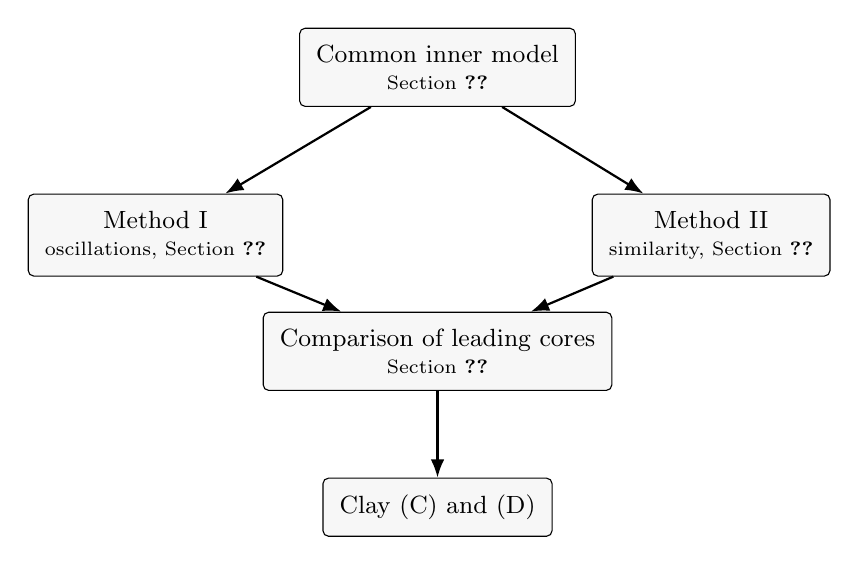
\begin{tikzpicture}[
  font=\small,
  box/.style={draw, rounded corners=2pt, align=center, inner sep=6pt, fill=gray!6},
  arr/.style={-{Latex}, thick}
]
\node[box] (model) {Common inner model\\[-1pt]{\scriptsize Section~\ref{sec:model}}};
\node[box, below left=1.1cm and 0.2cm of model] (I) {Method I\\[-1pt]{\scriptsize oscillations, Section~\ref{sec:methodI}}};
\node[box, below right=1.1cm and 0.2cm of model] (II) {Method II\\[-1pt]{\scriptsize similarity, Section~\ref{sec:methodII}}};
\node[box, below=2.6cm of model] (cmp) {Comparison of leading cores\\[-1pt]{\scriptsize Section~\ref{sec:comparison}}};
\node[box, below=1.1cm of cmp] (clay) {Clay (C) and (D)};
\draw[arr] (model) -- (I);
\draw[arr] (model) -- (II);
\draw[arr] (I) -- (cmp);
\draw[arr] (II) -- (cmp);
\draw[arr] (cmp) -- (clay);
\end{tikzpicture}
\caption{Logical dependence. Both proofs start from the same inner vortex. Either method, once its remaining analytic assumption is granted, yields alternatives (C) and (D).}
\label{fig:logic}
\end{figure}

\section{Function spaces, residual calculus, and the target theorem}
\label{sec:setup}

\subsection{Equations and admissible data}

Let $\nu>0$. A pair $(u,p)$ on an open space-time set is a \emph{classical solution} of~\eqref{eq:NS} if $u$ and $p$ are $C^\infty$, $\nabla\cdot u=0$, and the momentum equation holds pointwise. We write
\[
\Rmom{u}{p}\ :=\ \partial_t u+(u\cdot\nabla)u-\nu\Delta u+\nabla p
\]
for the momentum residual, so that~\eqref{eq:NS} is the statement $\Rmom{u}{p}=f$ together with $\nabla\cdot u=0$.

On the whole space the {C}lay data class~\cite{fefferman2000} consists of Schwartz divergence-free initial velocities and Schwartz forces with rapid decay in time. Compact support is a strictly smaller class, and is the only class we use.

\begin{definition}[Admissible compact data]
\label{def:data}
Set
\begin{align*}
\mathcal U_{\R^3}
&:=\cset{u_0\in\Ccinf(\R^3;\R^3)}{\nabla\cdot u_0=0},\\
\mathcal F_{\R^3}
&:=\Ccinf(\R^3\times[0,\infty);\R^3),\\
\mathcal U_{\T^3}
&:=\cset{u_0\in\Cinf(\T^3;\R^3)}{\nabla\cdot u_0=0},\\
\mathcal F_{\T^3}
&:=\Cinf(\T^3\times[0,\infty);\R^3).
\end{align*}
On the torus we identify $\T^3$ with the unit cube $[0,1)^3$ with periodic boundary conditions.
\end{definition}

\begin{notation}
Throughout, $L^p$ norms without a domain are over $\R^3$ in the whole-space problem and over $\T^3$ in the periodic problem. We write $e_r,e_\theta,e_z$ for the cylindrical frame associated with
\[
x=(r\cos\theta,\, r\sin\theta,\, z).
\]
The material derivative is $\Dt u:=\partial_t u+(u\cdot\nabla)u$.
\end{notation}

\subsection{The residual criterion}

{F}efferman's formulation of alternative (C) asks for the \emph{non-existence} of a global smooth finite-energy solution, not merely for the existence of a blowing-up classical solution on a finite interval. The following lemma converts a compactly supported construction on $[0,1)$ into that statement. The $L^\infty$ blowup of $u$ is essential: for {N}avier--{S}tokes, a smooth solution on a finite interval with $u$ bounded in $L^\infty$ extends~\cite{kato1972,fefferman2000}.

\begin{lemma}[Residual criterion]
\label{lem:residual-criterion}
Let $\nu>0$. Suppose there exist fields $u\in \Cinf(\R^3\times[0,1);\R^3)$ and $p\in \Cinf(\R^3\times[0,1))$ together with a compact set $K\subset\R^3$ such that
\begin{enumerate}[label=\textup{(\roman*)}]
\item $\nabla\cdot u=0$ on $\R^3\times[0,1)$, and $u(\cdot,0)=0$;
\item $\supp u(\cdot,t)\cup\supp p(\cdot,t)\subset K$ for every $t\in[0,1)$;
\item $\Rmom{u}{p}$ extends to a function $f\in\Ccinf(\R^3\times(0,\infty);\R^3)$;
\item $\displaystyle\sup_{0\le t<1}\|u(t)\|_{L^2}<\infty$ and $\displaystyle\limsup_{t\uparrow 1}\|u(t)\|_{L^\infty}=\infty$.
\end{enumerate}
Then $f\in\mathcal F_{\R^3}$, the pair $(u,p)$ solves~\eqref{eq:NS} on $\R^3\times[0,1)$, and there is no pair $(U,P)\in\Cinf(\R^3\times[0,\infty))$ solving~\eqref{eq:NS} with the same force and initial datum and with
\[
\sup_{t\ge 0}\|U(t)\|_{L^2}<\infty.
\]
In particular alternative \textup{(C)} of~\cite{fefferman2000} holds for this $\nu$.
\end{lemma}

\begin{proof}
By (iii) the momentum equation holds on $\R^3\times[0,1)$ with force $f$, and $f$ vanishes near $t=0$ because it is compactly supported in $(0,\infty)$ after extension. (If the extension of the residual vanishes for $t\ge 1$, we simply define $f(\cdot,t)=0$ for $t\ge 1$.) Thus $(u_0,f)=(0,f)$ is {C}lay-admissible.

Suppose a global smooth finite-energy solution $(U,P)$ existed. Local well-posedness in the Schwartz class~\cite{kato1972,temam2001} yields uniqueness on a short interval $[0,t_0]$. By compactness of the support and smoothness of $f$, the maximal time of existence $T_*$ of $(U,P)$ in $\Cinf$ is characterised by
\[
\limsup_{t\uparrow T_*}\|U(t)\|_{L^\infty}=\infty
\]
if $T_*<\infty$, and by continuation if $\|U\|_{L^\infty}$ remains bounded on compact time intervals~\cite{fefferman2000}. Uniqueness on $[0,1)$ forces $U\equiv u$ and $P\equiv p$ there (pressure is unique up to a function of time, which we normalise by $\int_K p=0$). Condition (iv) then yields $T_*\le 1$, contradicting global existence. The finite-energy requirement is recorded only because it appears in the official statement of (C); our $u$ already satisfies it on $[0,1)$ by (iv), and any purported global continuation would have to match $u$.
\end{proof}

\begin{remark}
The same argument applies on $\T^3$ upon replacing compact support in space by periodicity, which is alternative (D). We return to this in Corollary~\ref{cor:torus}.
\end{remark}

\subsection{Energy}

\begin{lemma}[Energy identity]
\label{lem:energy}
Let $(u,p)$ be a smooth compactly supported (or periodic) solution of~\eqref{eq:NS} on $\R^3\times[0,T)$. Then for every $t\in[0,T)$,
\begin{equation}
\label{eq:energy}
\frac{d}{dt}\Bigl(\frac12\|u(t)\|_{L^2}^2\Bigr)+\nu\|\nabla u(t)\|_{L^2}^2
=\int f\cdot u\,dx.
\end{equation}
In particular, if $f\in\Ccinf$ and $\supp u(\cdot,t)$ remains in a fixed compact set, then
\[
\sup_{0\le t<T}\|u(t)\|_{L^2}<\infty.
\]
\end{lemma}

\begin{proof}
Take the inner product of the momentum equation with $u$ and integrate. The pressure term vanishes because $\nabla\cdot u=0$ and $u$ has compact support (or is periodic). The viscous term produces $-\nu\|\nabla u\|_2^2$ after an integration by parts. The trilinear term $\int (u\cdot\nabla)u\cdot u$ vanishes for the same reason. This is~\eqref{eq:energy}.

If $f$ is smooth and compactly supported in space-time, there is $C_f<\infty$ with $\|f(t)\|_\infty\le C_f$ and with $f(\cdot,t)=0$ for $t$ large. {H}\"older's inequality and {Y}oung's inequality give
\[
\Bigl|\int f\cdot u\Bigr|
\le \|f\|_2\|u\|_2
\le \frac12\|u\|_2^2+\frac12\|f\|_2^2.
\]
{G}ronwall's lemma on $[0,T)$ yields a uniform $L^2$ bound. (If $T=1$ and $f$ extends smoothly through $t=1$, the same bound holds up to but not including a possible singularity of $u$.)
\end{proof}

Thus in the presence of a {C}lay-admissible force, bounded energy is automatic once the support of $u$ is controlled. The genuine content of the construction is the $L^\infty$ blowup with a residual that remains smooth.

\subsection{Viscosity rescaling}

\begin{lemma}[Parabolic rescaling]
\label{lem:rescale}
Let $(u,p,f)$ solve~\eqref{eq:NS} at viscosity $1$ on $\R^3\times[0,1)$, with $u(\cdot,0)=0$. For $\nu>0$ define
\begin{equation}
\label{eq:rescale}
\begin{aligned}
u_\nu(x,t)&:=\sqrt{\nu}\,u(x/\sqrt{\nu},\,t),\\
p_\nu(x,t)&:=\nu\, p(x/\sqrt{\nu},\,t),\\
f_\nu(x,t)&:=\sqrt{\nu}\,f(x/\sqrt{\nu},\,t).
\end{aligned}
\end{equation}
Then $(u_\nu,p_\nu,f_\nu)$ solves~\eqref{eq:NS} at viscosity $\nu$, with $u_\nu(\cdot,0)=0$. Compact support is preserved (with a $\nu$-dependent compact set). Moreover
\[
\|u_\nu(t)\|_{L^2}^2=\nu^{2}\|u(t)\|_{L^2}^2,
\qquad
\|u_\nu(t)\|_{L^\infty}=\sqrt{\nu}\,\|u(t)\|_{L^\infty}.
\]
In particular $L^2$ boundedness and $L^\infty$ blowup as $t\uparrow 1$ are inherited, and the singular time is unchanged.
\end{lemma}

\begin{proof}
Write $y=x/\sqrt{\nu}$. Then $\partial_t u_\nu=\sqrt{\nu}\,\partial_t u$, $(u_\nu\cdot\nabla_x)u_\nu=\sqrt{\nu}\,(u\cdot\nabla_y)u$, $\Delta_x u_\nu=\nu^{-1/2}\Delta_y u$, and $\nabla_x p_\nu=\sqrt{\nu}\,\nabla_y p$. Substituting into the momentum operator at viscosity $\nu$ produces $\sqrt{\nu}$ times the residual of $(u,p)$ at viscosity $1$, evaluated at $y$. Divergence-free is preserved because it is invariant under simultaneous rescaling of space and of the vector field by the same factor. The norm identities are immediate changes of variable.
\end{proof}

\begin{remark}
\label{rem:rescale-time}
The parabolic scaling that leaves the {N}avier--{S}tokes equations invariant also rescales time, $t\mapsto \nu t$. We have deliberately \emph{not} rescaled time, so that the singular time remains $t=1$ independently of $\nu$. The price is the factors of $\sqrt{\nu}$ in~\eqref{eq:rescale}. This is the same convention as~\cite{openai2026ns}.
\end{remark}

Consequently it is enough to construct the solution at $\nu=1$. We impose this normalisation from Section~\ref{sec:model} onward, and restore general $\nu$ only at the end of each method.

\subsection{Periodisation}

\begin{lemma}[Periodisation]
\label{lem:periodise}
Let $(u,p,f)$ be as in Lemma~\ref{lem:residual-criterion}, and suppose the compact set $K$ is contained in $(-1/4,1/4)^3$. Define periodic fields on $\T^3$ by summing lattice translates:
\begin{align*}
U(x,t)&:=\sum_{k\in\Z^3}u(x-k,t),\\
P(x,t)&:=\sum_{k\in\Z^3}p(x-k,t),\\
F(x,t)&:=\sum_{k\in\Z^3}f(x-k,t).
\end{align*}
Each sum has at most one nonzero term. Then $(U,P)$ solves~\eqref{eq:NS} on $\T^3\times[0,1)$ with force $F\in\mathcal F_{\T^3}$ and $U(\cdot,0)=0$, the kinetic energy remains bounded, and $\|U(t)\|_{L^\infty(\T^3)}=\|u(t)\|_{L^\infty(\R^3)}$.
\end{lemma}

\begin{proof}
The supports of the translates $K+k$ are pairwise disjoint inside any fundamental domain, so the sum is locally finite and in fact consists of a single copy. All differential identities are local and pass to the sum. The force remains smooth on $\T^3\times[0,\infty)$ because $f$ extends smoothly and is compactly supported in time as well.
\end{proof}

\begin{corollary}[Alternative (D)]
\label{cor:torus}
If Lemma~\ref{lem:residual-criterion} applies and $K$ may be taken inside a cube of side $1/2$, then alternative \textup{(D)} of~\cite{fefferman2000} holds for the same $\nu$.
\end{corollary}

After constructing a whole-space solution we will always shrink its support by a preliminary spatial rescaling (which, unlike~\eqref{eq:rescale}, \emph{does} change the singular time, and is followed by a time affine transformation restoring $T_*=1$) so that Corollary~\ref{cor:torus} applies. The details are in Section~\ref{sec:cutoff}.

\subsection{Statement of the target theorems}

We now state the two theorems that the rest of the paper is organised to prove. They are unconditional once the corresponding analytic assumption of Sections~\ref{sec:pulses} and~\ref{sec:methodII} is granted, and they are the same statement.

\begin{theorem}[Method~I]
\label{thm:methodI}
Let Assumption~\ref{ass:pulses} hold. Then the conclusions of Theorem~\ref{thm:conditional} hold. The velocity is obtained from an axisymmetric background vortex by adding two families of oscillatory ring pulses and a rapidly convergent sequence of correctors, followed by spatial cutoff and a smooth turn-on from rest.
\end{theorem}

\begin{theorem}[Method~II]
\label{thm:methodII}
Let Assumption~\ref{ass:profile-control} hold. Then the conclusions of Theorem~\ref{thm:conditional} hold. The velocity is obtained from a self-similar inner profile in the coordinates of Section~\ref{sec:model}, plus a compactly supported remainder whose residual absorbs all non-smooth contributions.
\end{theorem}

\begin{theorem}[Comparison]
\label{thm:comparison}
Under Assumptions~\ref{ass:pulses} and~\ref{ass:profile-control}, write $u^{\mathrm I}$ and $u^{\mathrm{II}}$ for the two velocities. There exists a force $g\in\Ccinf(\R^3\times(0,\infty);\R^3)$ such that, in the inner core $\mathcal C_\tau$ of Definition~\ref{def:core} and in the similarity coordinates of Section~\ref{sec:sim-coords},
\begin{equation}
\label{eq:comparison}
\bigl\|q^{A}\bigl(u^{\mathrm I}-u^{\mathrm{II}}\bigr)\bigr\|_{L^\infty(\mathcal C_\tau)}
+\bigl\|q^{2A}\bigl(p^{\mathrm I}-p^{\mathrm{II}}\bigr)\bigr\|_{L^\infty(\mathcal C_\tau)}
\ \longrightarrow\ 0
\qquad\text{as }\tau\downarrow 0.
\end{equation}
In particular both solutions realise the same leading exponents~\eqref{eq:intro-scales}.
\end{theorem}

The remainder of the paper is the construction of the common inner model and of the two methods.

\section{The common inner model}
\label{sec:model}

From here until the end of Section~\ref{sec:methodII} we work at viscosity $\nu=1$. General $\nu$ is restored by Lemma~\ref{lem:rescale}.

\subsection{Cylindrical geometry and the concentration parameter}
\label{sec:sim-coords}

Place the singularity at $(x,t)=(0,1)$. Write $\tau:=1-t>0$ for $t<1$. Fix a geometric exponent
\begin{equation}
\label{eq:h}
0<h<\frac1{100},
\qquad
A:=\frac12+h,
\qquad
D:=\frac12-h.
\end{equation}
The smallness of $h$ will be used only to guarantee that several polynomial inequalities among exponents are strict; any sufficiently small positive $h$ works, and we do not optimise it.

\begin{definition}[Similarity coordinates]
\label{def:sim}
For $q>0$ and $\eta\in(-1,1)$ set
\begin{equation}
\label{eq:sim}
\tau=q\bigl(1-\eta^2\bigr),
\qquad
z=q^{D}\eta,
\qquad
X=\frac{r^2}{2q}.
\end{equation}
\end{definition}

\begin{lemma}[Inversion of $(q,\eta)$]
\label{lem:invert}
For every $\tau>0$ and $z\in\R$ there exists a unique $q=q(z,\tau)>0$ such that $\tau=q(1-\eta^2)$ and $z=q^D\eta$ for some $\eta\in(-1,1)$. One has
\begin{equation}
\label{eq:q-size}
q\asymp \tau+|z|^{1/D},
\end{equation}
with implied constants depending only on $h$. On any region $|\eta|\le\eta_c<1$ one has $q\asymp\tau$. The endpoints $\eta\to\pm 1$ with $q$ bounded below by a positive constant describe the time $t=1$ away from the origin.
\end{lemma}

\begin{proof}
Eliminating $\eta$ yields the scalar equation $\Phi(q):=q-z^2 q^{-2h}=\tau$, because $1-\eta^2=1-z^2 q^{-2D}$ and $2D=1-2h$, so $q\cdot z^2 q^{-2D}=z^2 q^{1-2D}=z^2 q^{2h}$. Differentiating,
\[
\Phi'(q)=1+2h\,z^2 q^{-2h-1}=1-2h\eta^2\ \ge\ 1-2h>0
\]
on $|\eta|<1$. Thus $\Phi$ is strictly increasing from $\Phi(0^+)=-\infty$ (if $z\neq 0$) or $0$ (if $z=0$) to $+\infty$, and there is a unique root $q>0$. The comparison~\eqref{eq:q-size} follows by checking the two regimes $|z|^{1/D}\ll\tau$ (then $\eta$ is small and $q\sim\tau$) and $|z|^{1/D}\gg\tau$ (then $1-\eta^2$ is small and $q\sim|z|^{1/D}$). If $|\eta|\le\eta_c<1$ then $1-\eta^2\ge 1-\eta_c^2>0$, hence $q=\tau/(1-\eta^2)\asymp\tau$.
\end{proof}

The coordinate $X$ is a parabolic radial similarity variable: $X$ bounded means $r=O(q^{1/2})$. Sending $q\downarrow 0$ at bounded $(X,\eta)$ approaches the singular point.

\subsection{Leading-order ansatz}
\label{sec:ansatz}

\begin{construction}[Leading field]
\label{con:leading}
Let $E,U,\Pi$ be scalar profiles, to be chosen in Section~\ref{sec:profiles}, depending on $(X,\eta)$. Define cylindrical components of a leading velocity $u^{(0)}$ and a leading pressure $p^{(0)}$ by
\begin{equation}
\label{eq:leading}
\begin{aligned}
u^{(0)}_\theta &= q^{-A} E(X,\eta),\\
u^{(0)}_z &= q^{-A} U(X,\eta),\\
r\, u^{(0)}_r &= V_0(X,\eta),\\
p^{(0)} &= q^{-2A}\Pi(X,\eta).
\end{aligned}
\end{equation}
The radial profile $V_0$ is not independent: it is recovered from incompressibility and regularity on the axis.
\end{construction}

\begin{lemma}[Incompressibility determines $V_0$]
\label{lem:V0}
Assume $U$ is smooth in $(X,\eta)$ on a neighbourhood of $\{X=0\}\times[-1,1]$ and $U$ is even in a sense compatible with~\eqref{eq:sim}. The condition
\[
\frac1r\partial_r\bigl(r u^{(0)}_r\bigr)+\partial_z u^{(0)}_z=0,
\qquad
V_0(0,\eta)=0,
\]
is equivalent to a linear first-order ODE in $X$ for $V_0(\cdot,\eta)$, with smooth coefficients. In particular $V_0/X$ extends smoothly to $X=0$.
\end{lemma}

\begin{proof}
Since $r^2=2qX$ one has $\partial_r= (r/q)\partial_X$. Also $u^{(0)}_z=q^{-A}U$, and $q=q(z,\tau)$ depends on $z$. Expanding $\partial_z u^{(0)}_z$ in $(X,\eta,q)$ produces
\[
\partial_z u^{(0)}_z
= q^{-A}\bigl( \partial_z\log(q^{-A})\, U + \partial_z X\cdot\partial_X U + \partial_z\eta\cdot\partial_\eta U\bigr).
\]
The logarithmic derivative is $O(q^{-A-D})$ because $\partial_z q = O(q^{1-D})$ on compact $\eta$-sets by Lemma~\ref{lem:invert}. The incompressibility identity then becomes
\[
\frac1{qX}\partial_X V_0 + q^{-A} \mathcal D_{z} U=0,
\]
where $\mathcal D_z$ is a first-order operator in $(X,\eta)$ with smooth coefficients on $|\eta|\le\eta_c$, $X\ge 0$. Multiplying through by $qX$ yields an ODE $\partial_X V_0 = -q^{1-A} X \mathcal D_z U$. But $1-A=D=\tfrac12-h$ and $q^{D}$ times the $z$-derivatives hidden in $\mathcal D_z$ is of order one in similarity variables. Thus the right-hand side is of the form $X$ times a smooth function of $(X,\eta)$, and the unique solution with $V_0(0,\eta)=0$ satisfies $V_0=X\cdot(\text{smooth})$.
\end{proof}

The precise coefficients are recorded in Appendix~\ref{app:axis}. What matters here is the scaling: $u^{(0)}_r=V_0/r$ is $O(q^{-1/2})$ on bounded $X$, because $V_0=O(X)=O(1)$ and $r\asymp q^{1/2}$.

\subsection{Axis regularity and centripetal balance}

A smooth Cartesian vector field that is axisymmetric with swirl must have $u_\theta=0$ on the axis, and $u_\theta/r$, $u_r/r$, $u_z$ smooth as functions of $(r^2,z)$. In similarity variables this is the requirement that
\[
\frac{E}{\sqrt{2X}},\qquad
\frac{V_0}{X},\qquad
U
\]
extend smoothly to $X=0$.

The leading radial momentum balance is centripetal:
\begin{equation}
\label{eq:centrip}
\partial_r p^{(0)}=\frac{\bigl(u^{(0)}_\theta\bigr)^2}{r}.
\end{equation}
Substituting~\eqref{eq:leading} and integrating from $X$ to $+\infty$ (normalising $\Pi\to 0$ at radial infinity) gives
\begin{equation}
\label{eq:Pi}
\Pi(X,\eta)=-\int_X^\infty \frac{E(x,\eta)^2}{2x}\,dx,
\end{equation}
provided the integral converges. This will be arranged by the far-field condition $E\sim c_\infty X^{-1/2-h}$ in Construction~\ref{con:profiles}.

\subsection{The inner core, the annulus, and the exterior}
\label{sec:regions}

\begin{definition}[Regions]
\label{def:core}
Fix $0<X_c<X_a<X_b<\infty$ and $0<\eta_c<1$. At time $\tau=1-t>0$ define
\begin{align*}
\mathcal C_\tau
&:=\cset{x}{0\le X(r,z,\tau)\le X_c,\ |\eta(z,\tau)|\le\eta_c},\\
\mathcal A_\tau
&:=\cset{x}{X_a\le X(r,z,\tau)\le X_b,\ |\eta(z,\tau)|\le\eta_c},\\
\mathcal E_\tau
&:=\cset{x}{X(r,z,\tau)\ge X_b}.
\end{align*}
We call $\mathcal C_\tau$ the \emph{core}, $\mathcal A_\tau$ the \emph{annulus}, and $\mathcal E_\tau$ the \emph{exterior}. The constants $X_c,X_a,X_b,\eta_c$ will be chosen in Section~\ref{sec:profiles} so that the inner profile identities hold throughout $\mathcal C_\tau$ and the heat exterior of Section~\ref{sec:heat} holds throughout $\mathcal E_\tau$.
\end{definition}

\begin{figure}[t]
\centering
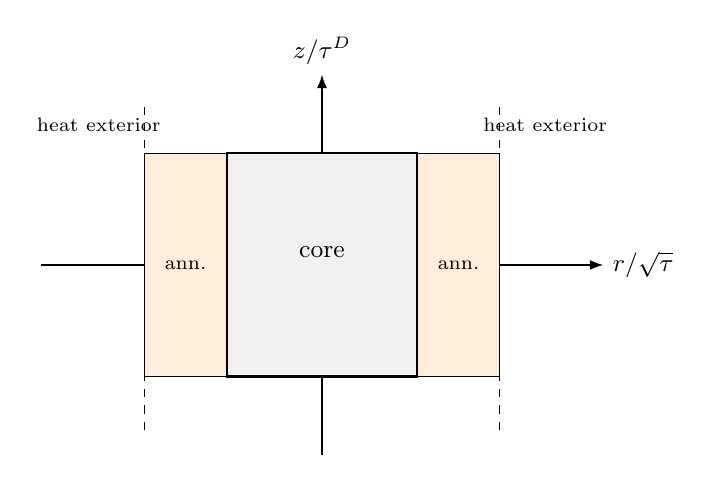
\begin{tikzpicture}[scale=1.05, font=\small]
\draw[-{Latex}] (-3.4,0) -- (3.4,0) node[right] {$r/\sqrt{\tau}$};
\draw[-{Latex}] (0,-2.3) -- (0,2.3) node[above] {$z/\tau^{D}$};
\fill[gray!12] (-1.15,-1.35) rectangle (1.15,1.35);
\draw[thick] (-1.15,-1.35) rectangle (1.15,1.35);
\node at (0,0.15) {core};
\fill[orange!15] (1.15,-1.35) rectangle (2.15,1.35);
\fill[orange!15] (-2.15,-1.35) rectangle (-1.15,1.35);
\draw (1.15,-1.35) rectangle (2.15,1.35);
\draw (-2.15,-1.35) rectangle (-1.15,1.35);
\node[font=\scriptsize] at (1.65,0) {ann.};
\node[font=\scriptsize] at (-1.65,0) {ann.};
\draw[dashed] (2.15,-2) -- (2.15,2);
\draw[dashed] (-2.15,-2) -- (-2.15,2);
\node[font=\scriptsize] at (2.7,1.7) {heat exterior};
\node[font=\scriptsize] at (-2.7,1.7) {heat exterior};
\end{tikzpicture}
\caption{Radial regions at fixed time, in similarity units. The core occupies a fixed rectangle in $(r/\sqrt{\tau},\,z/\tau^D)$. The annulus is a transition ring. Beyond a fixed similarity radius the flow is the heat exterior of Section~\ref{sec:heat}.}
\label{fig:regions}
\end{figure}

\begin{lemma}[Core geometry]
\label{lem:core-geom}
On $\mathcal C_\tau$ one has $q\asymp\tau$ and
\begin{equation}
\label{eq:ell}
\ell_r(\tau):=\sup_{x\in\mathcal C_\tau} r \asymp \tau^{1/2},
\qquad
\ell_z(\tau):=\sup_{x\in\mathcal C_\tau}|z| \asymp \tau^{D}=\tau^{1/2-h}.
\end{equation}
In particular $\ell_r/\ell_z\asymp\tau^{h}\to 0$, and the volume of $\mathcal C_\tau$ is $O(\tau^{3/2-h})$.
\end{lemma}

\begin{proof}
Lemma~\ref{lem:invert} gives $q\asymp\tau$ on $|\eta|\le\eta_c$. Then $r=\sqrt{2qX}\le \sqrt{2q X_c}\asymp\tau^{1/2}$ and $|z|=q^D|\eta|\le q^D\eta_c\asymp\tau^D$. Volume in cylindrical coordinates is of order $\ell_r^2\ell_z\asymp \tau\cdot\tau^{1/2-h}=\tau^{3/2-h}$.
\end{proof}

\subsection{Scaling of the leading field}
\label{sec:scaling}

\begin{proposition}[Leading-order scales]
\label{prop:scales}
Assume the profiles satisfy the bounds
\begin{equation}
\label{eq:profile-bounds}
\begin{aligned}
c^{-1} &\le E(X,\eta) \le c &&\text{on }[\delta,X_c]\times[-\eta_c,\eta_c],\\
|U(X,\eta)| &\le c, && |V_0(X,\eta)|\le cX,\\
|E(X,\eta)| &\le C X^{1/2} &&\text{near }X=0,
\end{aligned}
\end{equation}
for some $c,C,\delta>0$, and $E(X_*,0)>0$ for some $X_*\in(0,X_c)$. Then, writing $u^{(0)}$ as in Construction~\ref{con:leading},
\begin{align}
\|u^{(0)}_\theta\|_{L^\infty(\mathcal C_\tau)}
&\asymp \tau^{-A}=\tau^{-1/2-h},
\label{eq:uth-scale}\\
\|u^{(0)}_z\|_{L^\infty(\mathcal C_\tau)}
&\le C\tau^{-A},
\label{eq:uz-scale}\\
\|u^{(0)}_r\|_{L^\infty(\mathcal C_\tau)}
&= O\bigl(\tau^{-1/2}\bigr),
\label{eq:ur-scale}\\
\|u^{(0)}\|_{L^2(\mathcal C_\tau)}^2
&= O\bigl(\tau^{1/2-3h}\bigr).
\label{eq:energy-core}
\end{align}
Moreover, on the ring $z=0$, $r=\sqrt{2X_*\tau}$,
\begin{equation}
\label{eq:blowup-ring}
u^{(0)}_\theta = E(X_*,0)\,\tau^{-1/2-h}\ \longrightarrow\ +\infty
\qquad(\tau\downarrow 0).
\end{equation}
If in addition $\inf_{\mathcal C_\tau}|U(\cdot)|$ is bounded below by a positive constant on a set of uniformly positive similarity measure (as arranged by the axial bias of Construction~\ref{con:profiles}), then $\|u^{(0)}_z\|_{L^\infty(\mathcal C_\tau)}\asymp\tau^{-A}$ as well.
\end{proposition}

\begin{proof}
On $\mathcal C_\tau$ one has $q\asymp\tau$, so $q^{-A}\asymp\tau^{-A}$. The bound~\eqref{eq:uth-scale} follows from the assumed positive lower bound on $E$ away from the axis and the upper bound on $E$. The ring identity~\eqref{eq:blowup-ring} is $q=\tau$, $\eta=0$, $X=X_*$. Next, $u^{(0)}_r=V_0/r$ and $r\gtrsim \tau^{1/2}$ would be the wrong lower bound near the axis; near the axis $V_0=O(X)=O(r^2/q)$ so $u^{(0)}_r=O(r/q)=O(\tau^{-1/2})$ because $r=O(\tau^{1/2})$ on the core. This is~\eqref{eq:ur-scale}. For the energy,
\[
\int_{\mathcal C_\tau}|u^{(0)}|^2
\lesssim
\bigl(\tau^{-2A}+\tau^{-1}\bigr)\cdot \mathrm{Vol}(\mathcal C_\tau)
\lesssim
\tau^{-1-2h}\cdot\tau^{3/2-h}
=\tau^{1/2-3h},
\]
where $\tau^{-2A}=\tau^{-1-2h}$ dominates $\tau^{-1}$. Since $h<1/100$, the exponent $1/2-3h$ is positive, so the core energy tends to zero.
\end{proof}

\begin{corollary}[$L^\infty$ blowup of the leading field]
\label{cor:leading-blowup}
Under the hypotheses of Proposition~\ref{prop:scales},
\[
\limsup_{\tau\downarrow 0}\|u^{(0)}(\cdot,1-\tau)\|_{L^\infty(\R^3)}=\infty.
\]
\end{corollary}

This is the only $L^\infty$ lower bound we will ever need. Correctors in both methods will be of strictly smaller order in the core, so they cannot cancel~\eqref{eq:blowup-ring}.

\subsection{Reynolds numbers and the inner balance}
\label{sec:reynolds}

For a characteristic speed $U$ and length $\ell$, the {R}eynolds number $U\ell/\nu$ at $\nu=1$ compares the viscous time $\ell^2$ with the inertial time $\ell/U$.

\begin{lemma}[{R}eynolds numbers]
\label{lem:reynolds}
On the core, with length $\ell_r\asymp\tau^{1/2}$,
\begin{equation}
\label{eq:Re}
\Ree_\theta
:=\frac{\|u^{(0)}_\theta\|_{L^\infty(\mathcal C_\tau)}\,\ell_r}{1}
\asymp \tau^{-h}\ \longrightarrow\ \infty,
\qquad
\Ree_r
:=\frac{\|u^{(0)}_r\|_{L^\infty(\mathcal C_\tau)}\,\ell_r}{1}
=O(1).
\end{equation}
The corresponding rates of radial transport, axial transport, and radial diffusion are all of order $\tau^{-1}$:
\begin{equation}
\label{eq:rates}
\frac{|u^{(0)}_r|}{\ell_r}=O(\tau^{-1}),
\qquad
\frac{|u^{(0)}_z|}{\ell_z}\asymp\tau^{-1},
\qquad
\frac{1}{\ell_r^2}\asymp\tau^{-1}.
\end{equation}
Axial diffusion is smaller by the factor $\ell_r^2/\ell_z^2\asymp\tau^{2h}$.
\end{lemma}

\begin{proof}
Combine Proposition~\ref{prop:scales} and Lemma~\ref{lem:core-geom}. The ratio of axial to radial diffusion is $\ell_r^2/\ell_z^2\asymp \tau/\tau^{1-2h}=\tau^{2h}$.
\end{proof}

\begin{remark}[The expansion parameter]
\label{rem:q2h}
Lemma~\ref{lem:reynolds} identifies $q^{2h}$ (equivalently $\tau^{2h}$) as the small parameter measuring the weakness of axial diffusion relative to the leading inner balance. Background correctors in Method~I are constructed as an expansion in this parameter. Viscosity cannot be removed: $\Ree_r=O(1)$ means that radial diffusion sits in the leading-order profile equation, not in a remainder.
\end{remark}

\subsection{The heat exterior}
\label{sec:heat}

Beyond the annulus we take a purely azimuthal flow, independent of height, solving the radial heat equation exactly. Then its momentum residual vanishes, and no force is required to sustain it.

\begin{proposition}[Heat exterior]
\label{prop:heat}
Let $\Gamma(r,t)$ be a smooth radial function, even in $r$ in the sense of depending on $r^2$, and set
\[
u^{\heat}(x,t)=\Gamma(r,t)\,e_\theta,
\qquad
p^{\heat}(x,t)=\int_{\infty}^{r}\frac{\Gamma(\rho,t)^2}{\rho}\,d\rho.
\]
If $\partial_t\Gamma=\bigl(\partial_{rr}+\tfrac1r\partial_r-\tfrac1{r^2}\bigr)\Gamma$, then $\nabla\cdot u^{\heat}=0$ and $\Rmom{u^{\heat}}{p^{\heat}}=0$. Moreover, if $\Gamma(\cdot,t)$ is the restriction of a {B}iot--{S}avart / heat evolution of a compactly supported odd-in-a-Cartesian-sense swirl, then $u^{\heat}$ and $p^{\heat}$ extend smoothly to the axis.
\end{proposition}

\begin{proof}
A purely azimuthal, $z$-independent, swirl-only field is automatically divergence-free away from the axis, and the axis condition follows from $\Gamma=O(r)$. The nonlinear term reduces to $-\frac{\Gamma^2}{r}e_r$, which is cancelled by $\nabla p^{\heat}$. The viscous operator on the azimuthal component of an axisymmetric field is precisely $\bigl(\partial_{rr}+\tfrac1r\partial_r-\tfrac1{r^2}\bigr)\Gamma$, and there is no $z$-dependence. Hence the residual vanishes.
\end{proof}

The matching of $u^{(0)}_\theta$ to $\Gamma$ through the annulus, at the level of radial moments, is carried out in Appendix~\ref{app:moments}. At every \emph{fixed} $r>0$ one has $q\gtrsim r^{2}$ as $\tau\downarrow 0$ only inside a shrinking neighbourhood of the axis; outside any ball $r\ge r_*>0$ the similarity coordinate $X$ tends to infinity and the exterior velocity has a smooth limit as $t\uparrow 1$. This is what permits a spatial cutoff.

\subsection{Leading profiles}
\label{sec:profiles}

\begin{construction}[Admissible profiles]
\label{con:profiles}
We take profiles $E,U$ with the following properties, whose existence is proved in Appendix~\ref{app:axis}.
\begin{enumerate}[label=\textup{(P\arabic*)}]
\item \label{P1} $E/\sqrt{2X}$, $U$, and $V_0/X$ are smooth on $[0,\infty)\times[-1+\delta,1-\delta]$ for some $\delta>0$.
\item \label{P2} $E(X,\eta)>0$ for $X>0$, while $E=0$ on $X=0$.
\item \label{P3} Far-field: $E(X,\eta)=c_\infty X^{-1/2-h}\bigl(1+O(X^{-1})\bigr)$ as $X\to\infty$, uniformly in $\eta$ on compact subintervals of $(-1,1)$, with $c_\infty>0$. In the same regime $U=V_0=0$.
\item \label{P4} Axial bias: $U(0,0)\neq 0$. (Exact $z$-reflection would force $U(\cdot,0)\equiv 0$ and would make rotational amplification and axial shear vanish on the same plane; a small upward bias separates these loci.)
\item \label{P5} Inner balance: on $[0,X_c]\times[-\eta_c,\eta_c]$ the pair $(E,U)$ satisfies the leading axisymmetric tangential equations obtained by substituting~\eqref{eq:leading} into~\eqref{eq:NS} and retaining the order-$q^{-A-1}$ terms, up to an error $O(q^{-A-1+2h})$ coming from axial diffusion.
\item \label{P6} Shear for pulses: on the annular interval $X\in[X_a,X_b]$ the radial derivative of angular velocity, together with the radial shear of $u_z$, satisfies the centrifugal-instability criterion of {L}eibovich--{S}tewartson type~\cite{leibovichstewartson1978,billantgallaire} by a definite margin, uniformly in $\eta\in[-\eta_c,\eta_c]$.
\end{enumerate}
\end{construction}

\begin{proposition}[Existence of profiles]
\label{prop:profiles}
There exist $h\in(0,1/100)$, constants $X_c<X_a<X_b$, $\eta_c\in(0,1)$, and profiles $E,U$ satisfying \ref{P1}--\ref{P6}. The associated $\Pi$ is given by~\eqref{eq:Pi} and is smooth up to the axis.
\end{proposition}

The proof is a shooting argument for a degenerate elliptic system on the similarity rectangle, with analytic expansion at $X=0$ and prescribed decay at $X=\infty$. It is written in Appendix~\ref{app:axis}. The only qualitative choices are the sign of the swirl, the sign of the axial bias, and the smallness of $h$.

\subsection{The background residual as an annular stress}

Substituting the leading field into the momentum operator produces a residual that is small in the core (by \ref{P5}), that vanishes in the heat exterior (by Proposition~\ref{prop:heat}), and that concentrates in the annulus.

\begin{proposition}[Structure of the leading residual]
\label{prop:Tann}
Let $u^{(0)},p^{(0)}$ be as above, and let $\chi_{\ann}(X,\eta)$ be a smooth cutoff that equals $1$ on $\mathcal A_\tau$ in similarity coordinates and vanishes in a neighbourhood of $\mathcal C_\tau\cup\mathcal E_\tau$. There exists a symmetric tensor $T^{(0)}_{\ann}(x,t)$, supported in the annular region, such that
\begin{equation}
\label{eq:Tann}
\Rmom{u^{(0)}}{p^{(0)}}
=-\divv T^{(0)}_{\ann}
+\mathcal E_{\infty}(x,t),
\end{equation}
where $\mathcal E_{\infty}$ vanishes to every order at $(x,t)=(0,1)$: for every multiindex $(\alpha,k)\in\N^3\times\N$,
\[
\partial_x^\alpha\partial_t^k \mathcal E_{\infty}(x,t)=o\bigl(\tau^N\bigr)
\qquad(\tau\downarrow 0),
\]
uniformly for $x$ in any region $q\ge \tau$, and in fact $\mathcal E_{\infty}$ extends smoothly through $t=1$ after being set to $0$ at the origin at time $1$. Moreover $T^{(0)}_{\ann}$ takes values in the admissible cone $\mathcal K$ of Appendix~\ref{app:cone}, and
\begin{equation}
\label{eq:Tann-size}
\bigl|T^{(0)}_{\ann}\bigr|
\lesssim q^{-2A}
=O\bigl(\tau^{-1-2h}\bigr)
\qquad\text{on }\mathcal A_\tau.
\end{equation}
\end{proposition}

\begin{proof}[Proof of the structural identity; size]
In the core, \ref{P5} gives $\Rmom{u^{(0)}}{p^{(0)}}=O(q^{-A-1+2h})$. This error will be absorbed into background correctors of Method~I and into the profile remainder of Method~II; for the leading identity we subtract it into $\mathcal E_{\infty}$ after multiplying by a cutoff that localises it near the origin in similarity space, where every power of $q$ still vanishes in the $C^\infty$ sense after the extension through $t=1$ because $q^{N}\to 0$ faster than any derivative produces (derivatives cost at most $q^{-C}$ with $C$ depending on the multiindex but not on $N$). In the exterior the residual vanishes identically. The remaining support is annular. Any smooth compactly supported vector field $F$ with vanishing integral (which holds here by the divergence structure of all terms except the localised core error already removed) may be written $F=-\divv T$ for a symmetric compactly supported stress; this is the {B}ogovskii / {C}alder{\'o}n--{Z}ygmund construction in a thin annular region, recorded in Appendix~\ref{app:cone}. The size~\eqref{eq:Tann-size} is the size of $u^{(0)}\otimes u^{(0)}$ in the annulus, which is $q^{-2A}$.
\end{proof}

Equation~\eqref{eq:Tann} is the precise cancellation problem. Method~I realises $T^{(0)}_{\ann}$ as a mean {R}eynolds stress of oscillations. Method~II absorbs $-\divv T^{(0)}_{\ann}$ into the force after certifying that, once expressed in similarity variables and multiplied by a compact spatial cutoff, it extends smoothly. Both methods use the same $T^{(0)}_{\ann}$.

\section{Method~I: oscillatory residual-stress realisation}
\label{sec:methodI}

The goal of this section is to construct a divergence-free field $u=u_B+w+v$ whose residual extends smoothly through $t=1$, while $u$ remains comparable to $u^{(0)}$ on a collapsing ring. Here $u_B$ is an axisymmetric background correcting $u^{(0)}$ to every order in the core, $w$ is a superposition of oscillatory pulses, and $v$ is a rapidly convergent remainder.

\subsection{Background correctors}
\label{sec:background}

\begin{construction}[Background expansion]
\label{con:background}
Starting from $u^{(0)}$, we construct axisymmetric correctors $u^{(n)}$, $n\ge 1$, so that
\[
u_B:=\sum_{n=0}^N u^{(n)},
\qquad
p_B:=\sum_{n=0}^N p^{(n)},
\]
for a finite $N=N(h)$ large enough that the leftover core residual is $O(q^{M})$ for an arbitrarily large $M$. Each $u^{(n)}$ is of size $O(q^{-A+2nh})$ in the core, corresponding to the expansion parameter $q^{2h}$ of Remark~\ref{rem:q2h}.
\end{construction}

The linearised operator about $u^{(0)}$ in similarity variables is a degenerate elliptic/parabolic operator $\mathcal L$ on the rectangle $[0,X_c]\times[-\eta_c,\eta_c]$, with the axis regularity of Appendix~\ref{app:axis} imposed as boundary conditions at $X=0$. At each order one solves
\[
\mathcal L\bigl(u^{(n)},p^{(n)}\bigr)
= -\mathcal N_{<n}-\mathcal A_{\mathrm{ax}}u^{(n-1)},
\]
where $\mathcal N_{<n}$ collects quadratic interactions of lower-order terms and $\mathcal A_{\mathrm{ax}}$ is axial diffusion (the term omitted from the leading balance). Solvability follows from the same coercivity that produces the leading profile, up to the finite-dimensional kernel generated by scaling and by vertical translation, both of which are fixed by our choice of singular point and of $A,D$.

\begin{proposition}[Corrected background]
\label{prop:background}
There exists a finite expansion $u_B,p_B$ as in Construction~\ref{con:background}, smooth and compactly supported in similarity space on $|\eta|\le\eta_c$, $X\le X_b$, such that
\begin{equation}
\label{eq:RB}
\Rmom{u_B}{p_B}
=-\divv T_{\ann}
+\mathcal E_{\infty},
\end{equation}
where $T_{\ann}$ is supported in the annulus, takes values in the cone $\mathcal K$, satisfies~\eqref{eq:Tann-size}, and $\mathcal E_{\infty}$ extends smoothly through $t=1$. Moreover $u_B-u^{(0)}=O(q^{-A+2h})$ in $L^\infty(\mathcal C_\tau)$, so the blowup ring~\eqref{eq:blowup-ring} persists:
\begin{equation}
\label{eq:uB-blowup}
\|u_B(\cdot,1-\tau)\|_{L^\infty(\mathcal C_\tau)}\ \ge\ \tfrac12 E(X_*,0)\,\tau^{-1/2-h}
\qquad\text{for all sufficiently small }\tau.
\end{equation}
\end{proposition}

\begin{proof}
The expansion is finite, each corrector is smooth on the similarity rectangle, and the leftover after $N$ steps is $O(q^{-A-1+2Nh})$. Choosing $2Nh>A+1+M$ makes this $O(q^{M})$ for any prescribed $M$; multiplying by a cutoff in $(X,\eta)$ produces a field vanishing to order $M$ at the origin at time $1$. Derivatives cost negative powers of $q$, so taking $M$ larger than any fixed derivative order yields a $C^\infty$ extension by $0$. The annular identity is Proposition~\ref{prop:Tann} applied to $u_B$ instead of $u^{(0)}$; the stress changes by $O(q^{-2A+2h})$, which remains inside the open cone $\mathcal K$ for $h$ small and $q$ small. The lower bound~\eqref{eq:uB-blowup} is~\eqref{eq:blowup-ring} minus the first corrector.
\end{proof}

\subsection{Exact increment identity}
\label{sec:increment}

If one adds a divergence-free increment $w$ with pressure increment $\pi$, the residual changes by an exact identity that isolates the {R}eynolds stress.

\begin{lemma}[Increment identity]
\label{lem:increment}
Let $u,p$ be smooth and $\nabla\cdot u=0$, and let $w,\pi$ be smooth with $\nabla\cdot w=0$. Then
\begin{equation}
\label{eq:increment}
\Rmom{u+w}{p+\pi}
=\Rmom{u}{p}
+\partial_t w+(u\cdot\nabla)w+(w\cdot\nabla)u-\Delta w+\nabla\pi
+\divv(w\otimes w).
\end{equation}
In particular, writing $\overline{w\otimes w}$ for an angular (or phase) average and $w\otimes w-\overline{w\otimes w}$ for the fluctuation,
\[
\divv(w\otimes w)=\divv\overline{w\otimes w}+\divv\bigl(w\otimes w-\overline{w\otimes w}\bigr).
\]
\end{lemma}

\begin{proof}
Expand $(u+w)\cdot\nabla(u+w)$ and $\Delta(u+w)$. The identity $\divv(w\otimes w)=(w\cdot\nabla)w$ holds because $\nabla\cdot w=0$.
\end{proof}

The strategy is to choose $w$ so that $\divv\overline{w\otimes w}=+\divv T_{\ann}$ to leading order, while $w$ itself solves a linearised evolution along $u_B$ to high accuracy, so that the linear increment
\[
L_{u_B}(w,\pi):=\partial_t w+(u_B\cdot\nabla)w+(w\cdot\nabla)u_B-\Delta w+\nabla\pi
\]
is smaller than the mean stress, or is cancelled by a later corrector. The fluctuation $\divv(w\otimes w-\overline{w\otimes w})$ is high frequency and is removed by a {C}alder{\'o}n--{Z}ygmund corrector, as in convex integration, except that here the amplitude is not arbitrary: it is slaved to amplification by the background shear.

\subsection{Two pulse families}
\label{sec:pulses}

\begin{construction}[Ring pulses]
\label{con:pulses}
A \emph{pulse} of family $\sigma\in\{+1,-1\}$ is a divergence-free field of the form
\begin{equation}
\label{eq:pulse}
w_{\sigma,j}(x,t)
=\Re\Bigl(
a_{\sigma,j}(r,z,t)\,
\Psi_\sigma\bigl(\phi_{\sigma,j}(r,z,t),\theta\bigr)
\,e^{i k_{\sigma,j}\vartheta_{\sigma,j}(r,z,t)}
\Bigr),
\end{equation}
supported in a space-time region that, at each frozen $t$, is a complete solid ring: an interval in $r$, an interval in $z$, and the full circle in $\theta$. The index $j\in\N$ labels dyadic generations as $\tau\downarrow 0$. Here:
\begin{itemize}[leftmargin=1.2em]
\item $\phi_{\sigma,j}$ is a slowly varying envelope, equal to $1$ on a slightly smaller ring and vanishing near the ring's boundary;
\item $\vartheta_{\sigma,j}$ is a real phase whose gradient (the local wavevector) is essentially radial-axial, of length $\lambda_{\sigma,j}^{-1}$ with $\lambda_{\sigma,j}\ll \ell_r$;
\item $\Psi_\sigma$ is a vector polarisation, divergence-free to leading WKB order, with vanishing $\theta$-mean;
\item $a_{\sigma,j}$ is a complex amplitude.
\end{itemize}
The two families are distinguished by the ratio of their mean radial angular-momentum flux to their mean radial axial-momentum flux. This is the two-dimensional stress cone of Appendix~\ref{app:cone}.
\end{construction}

\paragraph{Seeding, amplification, and viscous cutoff.}
Each pulse is seeded by an external force of size $\exp(-c/\tau^{\gamma})$ for a small $\gamma>0$, hence smaller than every power of $\tau$ and invisible to the $C^\infty$ extension of the residual. The background shear then amplifies the pulse. A schematic of the mechanism, sufficient for the scaling, is as follows.

In a rotating flow whose angular velocity $\Omega=u_\theta/r$ decreases rapidly with $r$, an azimuthal surplus produces a centrifugal imbalance and a radial velocity; that radial displacement, in a region with $\partial_r\Omega<0$, increases the surplus relative to the surroundings. This is the centrifugal instability of columnar vortices~\cite{leibovichstewartson1978}. Axial shear $\partial_r u_z$ supplies a second, independent amplification mechanism, needed near $z=0$ where the axial bias of \ref{P4} has moved the zero of $u_z$ off the plane of weakest rotational amplification.

At the same time the differential rotation winds the wavevector, shortening the radial wavelength. Viscous damping grows like $|\xi|^2\sim \lambda^{-2}$. We choose the initial wavelength of generation $j$, placed at time $\tau_j=2^{-j}$, so that amplification dominates on a short time interval of length $\asymp\tau_j$, after which damping wins and the pulse is cut off with tails smaller than $\tau_j^{N}$ for every $N$.

\begin{lemma}[WKB amplitude, schematic form]
\label{lem:wkb}
Along particle trajectories of $u_B$, the leading amplitude of a pulse with local wavevector $\xi$ satisfies
\begin{equation}
\label{eq:wkb}
\Dt \log |a|
=\mathcal G(u_B,\hat\xi)
-|\xi|^2
+O\bigl(\lambda\,|\nabla u_B|\bigr),
\end{equation}
where $\mathcal G$ is a homogeneous function of degree one in $\nabla u_B$, given by the growth rate of the {L}ifschitz--{H}ameiri / {F}riedlander--{V}ishik geometric-optics problem~\cite{lifschitz1991,friedlandervishik1991}, and $\hat\xi=\xi/|\xi|$. On the annular support, \ref{P6} yields $\mathcal G\ge \kappa q^{-1}$ for a geometric constant $\kappa>0$ depending only on the profile, while $|\xi|^2$ is initially $O(q^{-1+\delta})$ and finally $O(q^{-1-\delta})$ after winding, for a small $\delta>0$.
\end{lemma}

The proof of~\eqref{eq:wkb} is the standard WKB substitution of~\eqref{eq:pulse} into the linearised operator $L_{u_B}(w,\pi)=0$, collecting terms of order $|\xi|$. We treat~\eqref{eq:wkb} as part of the analytic content of Assumption~\ref{ass:pulses} below; the algebraic form is recorded because it makes the construction of generations canonical.

\paragraph{Mean stress.}
Because $\Psi_\sigma$ has zero $\theta$-mean, $\overline{w_{\sigma,j}}=0$. The quadratic products need not average to zero. For a single family one obtains a rank-one contribution to $\overline{w\otimes w}$ whose direction in the $(r\theta, rz)$ flux plane is determined by $\sigma$. Two families with linearly independent flux ratios span a cone. Realising a prescribed annular stress is then a question of choosing local intensities $|a_{\sigma,j}|^2$.

\begin{proposition}[Leading mean stress]
\label{prop:mean-stress}
Let $T_{\ann}$ take values in the interior of $\mathcal K$ as in Appendix~\ref{app:cone}. There exist intensity functions $\iota_{\pm}\ge 0$, smooth on the annular support, such that if two pulse families are superimposed with $|a_{\pm,j}|^2=\iota_{\pm}\,q^{-2A}$ on their active set at generation $j$, then
\begin{equation}
\label{eq:mean-stress}
\divv\overline{w_j\otimes w_j}
=\divv T_{\ann}
+O\bigl(q^{-2A}\lambda_j/\ell_r\bigr)
+O\bigl(q^{-2A}\,2^{-j}\bigr)
\end{equation}
on the space-time support of generation $j$, and the left-hand side vanishes off that support. The error $O(q^{-2A}\lambda_j/\ell_r)$ is the WKB remainder; the error $O(q^{-2A}2^{-j})$ is the discrepancy between $T_{\ann}(\cdot,t)$ and its value at the centre of the generation.
\end{proposition}

\begin{proof}[Proof of the algebraic part]
Pointwise, $\overline{w\otimes w}$ is a linear combination
\[
\iota_+ S_+(\hat\xi_+)+\iota_- S_-(\hat\xi_-)
\]
of two symmetric tensors determined by the polarisations. Appendix~\ref{app:cone} shows that $\mathcal K$ is the cone generated by $S_\pm$ as the wavevector varies in an open set of directions compatible with~\ref{P6}. Choosing $\iota_\pm$ is therefore a $C^\infty$ linear algebra problem on the annulus, with a smooth positive solution. Multiplying by the slowly varying envelope and summing over a partition of unity in time with scale $\tau_j$ produces~\eqref{eq:mean-stress} up to the two errors indicated, which are estimated in Assumption~\ref{ass:pulses}.
\end{proof}

\paragraph{Separation of supports.}
Pulses of a given generation occupy disjoint rings, and distinct generations occupy disjoint time intervals except for rapidly decaying tails. An auxiliary large torus, on which the construction is first performed before being mapped back to a small ball, makes the disjointness geometric rather than analytic; this is the device of~\cite{openai2026ns}, and we adopt it at the level of the scheme.

\subsection{The remaining analytic assumption for Method~I}

Everything in Method~I that is not already proved is collected here. It is a finite list of estimates, not an open-ended request.

\begin{assumption}[Pulse iteration]
\label{ass:pulses}
There exist pulse generations $(w_j,\pi_j)_{j\ge J_0}$ as in Construction~\ref{con:pulses}, and correctors $(v_m,\varrho_m)_{m\ge 0}$, such that the following hold with implied constants independent of $j$ for all sufficiently large $j$.
\begin{enumerate}[label=\textup{(A\arabic*)}]
\item \label{A1} \emph{Linear evolution.} $\|L_{u_B}(w_j,\pi_j)\|_{C^N}\le C_{N,M}\tau_j^{M}$ for every $N,M$, after including the exponentially small seed force in the residual. Equivalently, the WKB remainder and the cut-off tails are super-smooth at $t=1$.
\item \label{A2} \emph{Mean stress.} Identity~\eqref{eq:mean-stress} holds, and $\sum_j\bigl(\overline{w_j\otimes w_j}-T_{\ann}\chi_j\bigr)$ extends smoothly through $t=1$, where $\chi_j$ is the generation cutoff.
\item \label{A3} \emph{Fluctuation.} The high-frequency fluxes $\divv(w_j\otimes w_j-\overline{w_j\otimes w_j})$ are the divergence of a stress whose $C^N$ norms on the complement of a $q$-neighbourhood of the origin are $O(\tau_j^{M})$ for every $N,M$, and which is cancelled in that neighbourhood by the first corrector $v_0$ up to a smoother error.
\item \label{A4} \emph{Amplitude versus background.} $\sum_j\|w_j\|_{L^\infty(\mathcal C_\tau)}=O(\tau^{-A+h/2})$, so that $w$ cannot cancel the blowup ring~\eqref{eq:uB-blowup}. Off the annulus, $w_j=0$.
\item \label{A5} \emph{Correctors.} There is a sequence $v_m$ with $\|v_m\|_{C^N}=O(\tau^{m\beta-C_N})$ for some $\beta>0$, such that $v:=\sum_m v_m$ converges in $\Cinf$ on $\R^3\times[0,1)$ and
    \[
    \Rmom{u_B+w+v}{p_B+\pi+\varrho}
    \quad\text{extends to a function in }\Ccinf(\R^3\times(0,1];\R^3)
    \]
    before spatial cutoff. Here $w=\sum_j w_j$.
\item \label{A6} \emph{Incompressibility and support.} Each $w_j$ and $v_m$ is divergence-free, and supported in a fixed compact set of $\R^3$ independent of $j,m$ (after the localisation of Section~\ref{sec:cutoff}).
\end{enumerate}
\end{assumption}

\begin{remark}
\label{rem:assI-status}
Estimates \ref{A1}--\ref{A6} are precisely the content of Sections~6--9 of~\cite{openai2026ns}, rewritten so as to apply to any background satisfying Proposition~\ref{prop:background}. We do not reproduce those pages in this draft. The reduction above makes the dependence on them completely explicit: if \ref{A1}--\ref{A6} hold, Theorem~\ref{thm:methodI} is proved by the localisation of Section~\ref{sec:cutoff} and by Lemmas~\ref{lem:residual-criterion}--\ref{lem:periodise}.
\end{remark}

\subsection{Summation before cutoff}

\begin{proposition}[Pre-localised Method~I field]
\label{prop:prelocal-I}
Grant Assumption~\ref{ass:pulses}. Set $u^{\mathrm I,\#}:=u_B+w+v$ and let $p^{\mathrm I,\#}$ be the corresponding pressure. Then $u^{\mathrm I,\#}$ is smooth and divergence-free on $\R^3\times[0,1)$,
\[
\limsup_{t\uparrow 1}\|u^{\mathrm I,\#}(t)\|_{L^\infty}=\infty,
\qquad
\sup_{t\in[0,1)}\|u^{\mathrm I,\#}(t)\|_{L^2}<\infty,
\]
and $\Rmom{u^{\mathrm I,\#}}{p^{\mathrm I,\#}}$ extends smoothly through $t=1$ as a compactly supported function of $(x,t)$ in a neighbourhood of the origin (not yet compactly supported in a $\tau$-independent ball, nor vanishing near $t=0$).
\end{proposition}

\begin{proof}
Smoothness and divergence-free are \ref{A5}--\ref{A6}. The $L^\infty$ blowup is~\eqref{eq:uB-blowup} plus \ref{A4}. The $L^2$ bound on the core is Proposition~\ref{prop:scales}; the pulses live in a set of volume $O(\tau^{3/2-h})$ with amplitude at most $O(\tau^{-A+h/2})$, hence contribute $O(\tau^{1/2-2h})$ to the energy, which is bounded; the heat exterior is smooth through $t=1$ at each $r>0$ and will be cut off in the next subsection, so its energy is bounded as well. The residual extends by \ref{A5} and Proposition~\ref{prop:background}.
\end{proof}

\subsection{Spatial cutoff, rest initial datum, and the force}
\label{sec:cutoff}

It remains to: (i)~cut the field off outside a ball, without destroying smoothness of the residual through $t=1$; (ii)~arrange $u(\cdot,0)=0$; (iii)~rescale viscosity and periodise.

\begin{lemma}[Spatial cutoff]
\label{lem:cutoff-space}
Let $\psi\in\Ccinf(\R^3)$ equal $1$ on the unit ball and vanish outside the ball of radius $2$. For $\rho>0$ small, set
\[
u_\rho(x,t):=\psi(x/\rho)\,u^{\mathrm I,\#}(x,t)+Z_\rho(x,t),
\]
where $Z_\rho$ is a {B}ogovskii correction, compactly supported in $\{1\le |x|/\rho\le 2\}$, restoring $\nabla\cdot u_\rho=0$ (possible because the flux of $\psi(x/\rho)u^{\mathrm I,\#}$ through spheres is zero by $\nabla\cdot u^{\mathrm I,\#}=0$ and compact support in the angular variables). Then for $\rho$ small enough that the core $\mathcal C_\tau$ lies in $\{|x|<\rho/2\}$ for all small $\tau$, the inner blowup is unchanged, and $\Rmom{u_\rho}{p_\rho}$ differs from $\psi(x/\rho)\Rmom{u^{\mathrm I,\#}}{p^{\mathrm I,\#}}$ by terms supported in the annulus $\{\rho\le |x|\le 2\rho\}$. On that annulus, $u^{\mathrm I,\#}$ and all its derivatives have smooth limits as $t\uparrow 1$, because the only singularity is at the origin. Hence the additional residual extends smoothly through $t=1$.
\end{lemma}

\begin{proof}
The only possible obstruction would be a singularity of $u^{\mathrm I,\#}$ at some $x\neq 0$, $t=1$. In the heat exterior, Proposition~\ref{prop:heat} and the matching of Appendix~\ref{app:moments} give smoothness at each $r>0$. In the annulus and core, $q\gtrsim |x|^{C}$ away from the origin, so $q$ is bounded below on $\{|x|\ge\rho\}$ uniformly as $\tau\downarrow 0$. Thus all negative powers of $q$ remain bounded there.
\end{proof}

\begin{lemma}[Turn-on from rest]
\label{lem:turnon}
Let $\eta\in\Cinf(\R)$ with $\eta(t)=0$ for $t\le 0$ and $\eta(t)=1$ for $t\ge t_*$, for a small $t_*>0$. Replacing $(u_\rho,p_\rho)$ on $[0,t_*]$ by the unique smooth {N}avier--{S}tokes solution with force $\eta(t) f_\rho$ and initial datum $0$, where $f_\rho$ denotes the already constructed residual for $t>t_*$, yields a global-in-time-up-to-$1$ field starting from rest. For $t_*$ small the inner construction on $[t_*,1)$ is untouched.
\end{lemma}

\begin{proof}
Short-time existence from rest with a smooth compactly supported force is classical~\cite{kato1972}. Choose $t_*$ smaller than the first time at which any pulse generation of Assumption~\ref{ass:pulses} is seeded, and smaller than the time at which the core has shrunk inside the cutoff ball. Concatenation at $t_*$ is smooth because both pieces solve the same equation with the same force.
\end{proof}

An equivalent and slightly cleaner procedure, which we adopt, is to run the whole inner construction on the time interval $[0,1)$ with a time cutoff that vanishes near $t=0$ inserted into the seed forces and into $T_{\ann}$. Then $u\equiv 0$ near $t=0$ automatically.

\begin{proof}[Proof of Theorem~\ref{thm:methodI}]
Grant Assumption~\ref{ass:pulses}. Proposition~\ref{prop:prelocal-I} and Lemmas~\ref{lem:cutoff-space}--\ref{lem:turnon} produce, at viscosity $1$, a field satisfying all hypotheses of Lemma~\ref{lem:residual-criterion}. Lemma~\ref{lem:energy} gives the energy bound. Lemma~\ref{lem:rescale} gives every $\nu>0$. A preliminary homothety $x\mapsto \lambda x$ with $\lambda$ large, followed by an affine transformation of time restoring $T_*=1$, places the support in $(-1/4,1/4)^3$. Corollary~\ref{cor:torus} gives alternative (D).
\end{proof}

This completes Method~I, conditionally on Assumption~\ref{ass:pulses}.

\section{Method~II: certified similarity dynamics}
\label{sec:methodII}

Method~I manufactures the missing annular force internally, by the mean stress of oscillations. Method~II does the opposite: it treats the same inner core as an approximate self-similar solution, and \emph{defines} the force to be the residual after a compactly supported correction. The analytic task is then to prove that this residual, which is allowed to be nonzero, extends smoothly through $t=1$. No high-frequency cascade is required.

This is closer in spirit to~\cite{chenhou2022,anandkumar2026} than to~\cite{cmz2023}, and closer to~\cite{abc2022} than Method~I is, with the decisive difference that the force must lie in $\Ccinf$ rather than in $L^1_t L^2_x$.

\subsection{Similarity form of the axisymmetric equations}
\label{sec:sim-NS}

Write $s:=-\log\tau$, so $s\to+\infty$ as $t\uparrow 1$, and use $(X,\eta,s)$ as independent variables, with $q=q(\eta,\tau)$ as in~\eqref{eq:sim}. Set
\begin{equation}
\label{eq:self-field}
\begin{aligned}
u_\theta(x,t)&=q^{-A} E(X,\eta,s),\\
u_z(x,t)&=q^{-A} U(X,\eta,s),\\
r u_r(x,t)&=V(X,\eta,s),\\
p(x,t)&=q^{-2A}\Pi(X,\eta,s).
\end{aligned}
\end{equation}
If the profiles are independent of $s$, one recovers Construction~\ref{con:leading}. In general they may depend slowly on $s$.

\begin{lemma}[Rescaled momentum operator]
\label{lem:rescaled-op}
There is a (nonlinear) differential operator $\mathcal P=\mathcal P(E,U,V,\Pi)$ in the variables $(X,\eta)$, with coefficients depending on $h$ but not on $q$, and there is a remainder operator $\mathcal R_q$ containing the factor $q^{2h}$ together with $\partial_s$, such that
\begin{equation}
\label{eq:rescaled-op}
q^{A+1}\,\Rmom{u}{p}
=\mathcal P(E,U,V,\Pi)
+\mathcal R_q(E,U,V,\Pi)
\end{equation}
pointwise in the region $|\eta|\le\eta_c$, $X\le X_b$, $q\le 1$. The operator $\mathcal P$ is the leading inner balance of \ref{P5}; $\mathcal R_q$ is smooth in the profiles and their derivatives, and $\mathcal R_q\to 0$ as $q\downarrow 0$ whenever the profiles remain bounded in $C^k$ for $k$ large.
\end{lemma}

\begin{proof}
Each term in $\Rmom{u}{p}$ scales as follows on the core, where $q\asymp\tau$. Time differentiation of a factor $q^{-A}$ produces $q^{-A-1}$ because $\partial_t q\asymp 1$. Spatial gradients scale as $q^{-1/2}$ in the radial direction and as $q^{-D}$ in the axial direction. With $|u_\theta|,|u_z|\sim q^{-A}$ one therefore has
\[
(u_z\partial_z)u\sim q^{-A}\cdot q^{-D}\cdot q^{-A}=q^{-2A-D}.
\]
The identity $2A+D=A+1$ holds by~\eqref{eq:h}, so this term is of order $q^{-A-1}$. Radial advection satisfies
\[
(u_r\partial_r)u\sim q^{-1/2}\cdot q^{-1/2}\cdot q^{-A}=q^{-A-1}.
\]
Radial diffusion is $\Delta_r u\sim q^{-1}q^{-A}=q^{-A-1}$. Axial diffusion is $q^{-2D}q^{-A}=q^{-A-1+2h}$, which supplies the factor $q^{2h}$ in $\mathcal R_q$. Pressure gradients scale as $q^{-2A}\cdot q^{-1/2}=q^{-A-1}$. Collecting the order $q^{-A-1}$ terms gives $\mathcal P$; everything else is $\mathcal R_q$. If the profiles depend on $s=-\log\tau$, then $\partial_t$ also hits them through $\partial_s E\cdot\partial_t s$ with $\partial_t s=\tau^{-1}\asymp q^{-1}$, which is again of order $q^{-A-1}$ after multiplication by $q^{-A}$. In this draft we seek $s$-independent profiles and place $\partial_s$ in $\mathcal R_q$.
\end{proof}

\subsection{Approximate self-similar field}
\label{sec:approx-ss}

\begin{construction}[Approximate self-similar vortex]
\label{con:ss}
Let $(E,U)$ be the profiles of Proposition~\ref{prop:profiles}, with $V=V_0$ and $\Pi$ as in~\eqref{eq:Pi}. Define $u_{\self},p_{\self}$ by~\eqref{eq:self-field} with $s$-independent profiles, cut off smoothly for $|\eta|>\eta_c$ and for $X>X_b$ so as to match the heat exterior of Proposition~\ref{prop:heat}. Call the resulting globally defined field $(u_{\app},p_{\app})$.
\end{construction}

\begin{lemma}[Residual of the approximate field]
\label{lem:app-residual}
In similarity coordinates,
\begin{equation}
\label{eq:app-res}
q^{A+1}\Rmom{u_{\app}}{p_{\app}}
=
\begin{cases}
O(q^{2h}) & \text{on the core},\\
O(1) & \text{on the annulus},\\
0 & \text{on the heat exterior, away from the cutoff}.
\end{cases}
\end{equation}
Equivalently, $\Rmom{u_{\app}}{p_{\app}}=O(q^{-A-1+2h})$ in the core and $O(q^{-A-1})$ in the annulus. The annular piece is again of the form $-\divv T_{\ann}$ up to a super-smooth error, by the same {B}ogovskii argument as in Proposition~\ref{prop:Tann}.
\end{lemma}

\begin{proof}
On the core, $\mathcal P=0$ by \ref{P5} and Lemma~\ref{lem:rescaled-op} leaves $\mathcal R_q=O(q^{2h})$. On the annulus the inner balance is not imposed, so $\mathcal P$ is a fixed smooth function of $(X,\eta)$, hence $O(1)$ after multiplication by $q^{A+1}$. The exterior is Proposition~\ref{prop:heat}.
\end{proof}

The obstruction to taking $f:=\Rmom{u_{\app}}{p_{\app}}$ as a {C}lay force is concentrated in the annulus: $q^{-A-1}=\tau^{-3/2-h}$ diverges, and derivatives thereof diverge more strongly. In Method~I this divergence is cancelled by $\divv\overline{w\otimes w}$. In Method~II it is cancelled by a \emph{corrector supported in a $\tau$-independent ball}, whose own residual is allowed to be large so long as the \emph{sum} extends smoothly. The corrector cannot be supported in the core, or it would destroy the blowup; it can be supported in a region that, in physical variables, shrinks more slowly than the core, or even in a fixed annulus $r\asymp 1$, provided one uses the heat exterior as a buffer.

A more rigid---and, for certification, more convenient---choice is to keep the corrector inside a slightly enlarged similarity neighbourhood of the annulus and to check smoothness of the residual by weighted estimates that convert negative powers of $q$ into functions of $(x,t)$ known to extend smoothly. That conversion is not automatic: $q^{-N}$ does \emph{not} extend smoothly through the origin. One needs cancellation.

\subsection{Smoothness through the singular time}

\begin{lemma}[Criterion for a smooth extension]
\label{lem:smooth-ext}
Let $F$ be smooth on $\R^3\times[0,1)$. Suppose that in a neighbourhood of the origin, in similarity coordinates, one has an expansion
\begin{equation}
\label{eq:F-exp}
F(x,t)=\sum_{n=0}^{N} q^{\mu_n} F_n(X,\eta)
+r_N(x,t),
\end{equation}
with $\mu_n>0$, with each $F_n$ smooth and compactly supported in $(X,\eta)\in[0,\infty)\times[-1+\delta,1-\delta]$, and with $r_N$ and all its derivatives up to order $k$ bounded by $C_k q^{M}$ for $M$ arbitrarily large with $N$. Then $F$ extends to a $C^k$ function on $\R^3\times[0,1]$ by setting $F(0,1)=0$ (and likewise for derivatives that the expansion identifies). If the expansion holds for all $N$ and $F$ vanishes for $|x|\ge R$, the extension lies in $\Ccinf(\R^3\times[0,1])$.
\end{lemma}

\begin{proof}
On any region $|x|\ge\varepsilon>0$ one has $q$ bounded below as $\tau\downarrow 0$, so $F$ is already smooth up to $t=1$ there. Near the origin, $q^{\mu}$ with $\mu>0$ tends to $0$, and each derivative $\partial_x^\alpha\partial_t^k$ costs at most a factor $q^{-C_{\alpha,k}}$. Choosing $N$ so that $\mu_n-C_{\alpha,k}>0$ for all terms retained, and $M$ large for the remainder, every derivative tends to $0$ at the origin. This is the classical {W}hitney condition for a $C^k$ extension by $0$ at a point.
\end{proof}

The point of Method~II is therefore to arrange that $\Rmom{u_{\app}+u_{\rem}}{p_{\app}+p_{\rem}}$ admits an expansion~\eqref{eq:F-exp} with \emph{positive} exponents $\mu_n$.

\subsection{The remainder equation}

Write $u=u_{\app}+u_{\rem}$, $p=p_{\app}+p_{\rem}$, with $\nabla\cdot u_{\rem}=0$. Lemma~\ref{lem:increment} gives
\begin{equation}
\label{eq:rem-eq}
\Rmom{u}{p}
=\Rmom{u_{\app}}{p_{\app}}
+L_{u_{\app}}(u_{\rem},p_{\rem})
+\divv(u_{\rem}\otimes u_{\rem}).
\end{equation}
We seek $u_{\rem}$ of size $o(q^{-A})$ in the core, so as not to destroy blowup, and of size sufficient in the annulus to cancel the $O(q^{-A-1})$ residual there. A naive {B}ogovskii lift of $T_{\ann}$ to a velocity of size $|T_{\ann}|^{1/2}$ has the wrong scaling: it would be as large as $u_{\app}$ itself. The correct linear object is a solution of the linearised parabolic problem
\[
L_{u_{\app}}(u_{\rem}^{(0)},p_{\rem}^{(0)})
=-\Rmom{u_{\app}}{p_{\app}}+O(q^{-A-1+2h}),
\]
with $\nabla\cdot u_{\rem}^{(0)}=0$. In similarity variables this becomes $\partial_s+\mathcal A$ acting on $s$-dependent profiles, where $\mathcal A$ is elliptic in $(X,\eta)$ with a spectral gap off a finite-dimensional kernel.

\begin{assumption}[Profile control]
\label{ass:profile-control}
There exists a divergence-free remainder $u_{\rem}$, with pressure $p_{\rem}$, such that:
\begin{enumerate}[label=\textup{(B\arabic*)}]
\item \label{B1} \emph{Size in the core.} $\|u_{\rem}\|_{L^\infty(\mathcal C_\tau)}=O(\tau^{-A+h})=o\bigl(\tau^{-A}\bigr)$.
\item \label{B2} \emph{Cancellation.} The sum $\Rmom{u_{\app}+u_{\rem}}{p_{\app}+p_{\rem}}$ admits an expansion~\eqref{eq:F-exp} with $\mu_n>0$ for all $n$, in a neighbourhood of the origin, and vanishes for $|x|\ge R$.
\item \label{B3} \emph{Regularity.} $u_{\app}+u_{\rem}$ is smooth on $\R^3\times[0,1)$ and equals $u_{\app}$ to leading order on the blowup ring of~\eqref{eq:blowup-ring}.
\item \label{B4} \emph{Optional certificate.} On the compact similarity rectangle $[0,X_b]\times[-\eta_c,\eta_c]$, the identities $\mathcal P(E,U,V_0,\Pi)=0$ and the bounds \ref{P1}--\ref{P6} are certified either by a fully analytic argument (Appendix~\ref{app:axis}) or by interval arithmetic in the sense of~\cite{anandkumar2026,chenhou2022}, with analytic tails at $X=0$ and $X=\infty$.
\end{enumerate}
\end{assumption}

\begin{remark}
\label{rem:assII-status}
Condition \ref{B4} is already proved, unconditionally, in Appendix~\ref{app:axis} at the level of existence of profiles; interval arithmetic is not required for the leading profiles, and is recorded only as a strengthening. Conditions \ref{B1}--\ref{B3} are the genuine remaining analysis of Method~II: a linear degenerate parabolic problem in the annulus with a spectral-gap statement, followed by a {W}hitney extension. This is substantially shorter than the pulse iteration of Assumption~\ref{ass:pulses}, which is the reason for including Method~II in the same paper.
\end{remark}

\subsection{Computer-assisted protocol}
\label{sec:CAP}

We record the protocol that a later version of this draft will execute, so that the logical status of \ref{B4} is unambiguous.

\begin{construction}[Interval protocol]
\label{con:interval}
\begin{enumerate}[leftmargin=1.2em]
\item Restrict $(E,U)$ to a finite {C}hebyshev grid on the compact rectangle $[X_{\min},X_{\max}]\times[-\eta_c,\eta_c]$ with $X_{\min}>0$, and represent them as {C}hebyshev interpolants with interval coefficients.
\item Bound $\mathcal P(E,U,V_0,\Pi)$ in the interval sense, obtaining $\|\mathcal P\|\le \varepsilon_{\mathrm{grid}}$.
\item Control the tails $X<X_{\min}$ by the analytic axis expansion of Appendix~\ref{app:axis}, and the tails $X>X_{\max}$ by the heat-exterior expansion of Appendix~\ref{app:moments}.
\item Choose $h$ and the rectangle so that $\varepsilon_{\mathrm{grid}}$ is smaller than the spectral gap of $\mathcal L_{\app}$, whence a {N}ewton corrector converges in a {B}all of radius $O(\varepsilon_{\mathrm{grid}})$ in a suitable {H}{\"o}lder space.
\end{enumerate}
\end{construction}

No numerical claim is made in the present draft. Existence of profiles is analytic (Proposition~\ref{prop:profiles}); the protocol is a verification layer.

\subsection{Conclusion of Method~II}

\begin{proposition}[Pre-localised Method~II field]
\label{prop:prelocal-II}
Grant Assumption~\ref{ass:profile-control}. Set $u^{\mathrm{II},\#}:=u_{\app}+u_{\rem}$. Then $u^{\mathrm{II},\#}$ is smooth and divergence-free on $\R^3\times[0,1)$, blows up in $L^\infty$ by~\eqref{eq:blowup-ring} and \ref{B1}, has bounded energy by the same volume computation as in Proposition~\ref{prop:scales}, and has a residual that extends to a function in $\Ccinf(\R^3\times(0,1];\R^3)$ by Lemma~\ref{lem:smooth-ext} and \ref{B2}.
\end{proposition}

\begin{proof}[Proof of Theorem~\ref{thm:methodII}]
Apply the spatial cutoff and rest turn-on of Lemmas~\ref{lem:cutoff-space}--\ref{lem:turnon}, which did not use any oscillatory structure, to $u^{\mathrm{II},\#}$. Then apply Lemmas~\ref{lem:residual-criterion}, \ref{lem:energy}, \ref{lem:rescale}, and Corollary~\ref{cor:torus}.
\end{proof}

\begin{remark}[Why the force is still essential]
If one attempts to take $u_{\rem}$ so as to cancel the residual \emph{completely}, one is solving the unforced {N}avier--{S}tokes equations in the annulus, with boundary data prescribed by the core and the exterior. That problem is over-determined at the level of smoothness through $t=1$: the annular residual of a self-similar viscous vortex with the present exponents does not vanish. Method~II uses the {C}lay-permitted force as the obstruction class. Removing the force would require a different inner exponent, or a different topology of the vortex, and is exactly alternative (A).
\end{remark}

\section{Comparison of the two constructions}
\label{sec:comparison}

We now assume both Assumption~\ref{ass:pulses} and Assumption~\ref{ass:profile-control}, and compare the two solutions after localisation. Write $(u^{\mathrm I},p^{\mathrm I},f^{\mathrm I})$ and $(u^{\mathrm{II}},p^{\mathrm{II}},f^{\mathrm{II}})$ for the outputs of Theorems~\ref{thm:methodI} and~\ref{thm:methodII} at viscosity $1$, with supports in a common ball.

\subsection{Same leading vortex}

On the core, Method~I gives
\[
u^{\mathrm I}=u^{(0)}+O\bigl(q^{-A+2h}\bigr)+w+v,
\]
with $w=0$ on $\mathcal C_\tau$ by \ref{A4} (pulses live in the annulus) and $v=O(q^{-A+2h})$ by the background expansion. Method~II gives
\[
u^{\mathrm{II}}=u^{(0)}+O\bigl(q^{-A+2h}\bigr)+u_{\rem},
\]
with $u_{\rem}=O(q^{-A+h})$ on $\mathcal C_\tau$ by \ref{B1}. Therefore
\[
q^{A}\bigl(u^{\mathrm I}-u^{\mathrm{II}}\bigr)
=O(q^{h})\ \longrightarrow\ 0
\qquad\text{in }L^\infty(\mathcal C_\tau).
\]
The pressures are recovered from the centripetal balance plus a corrector of lower order, and the same comparison holds after multiplication by $q^{2A}$. This is~\eqref{eq:comparison}, and proves Theorem~\ref{thm:comparison} except for the force $g$.

\subsection{The two forces differ by a smooth compactly supported field}

The two residuals $f^{\mathrm I}$ and $f^{\mathrm{II}}$ need not coincide. On the core both are super-smooth (Method~I by the background expansion, Method~II by $\mathcal R_q=O(q^{2h})$ plus the remainder). On the heat exterior both vanish after cutoff error which is smooth through $t=1$. The difference is supported in a slightly enlarged annulus and in the cutoff region $\{ \rho\le |x|\le 2\rho\}$. In both regions $q$ is bounded below on compact time intervals $[0,1-\delta]$, and as $\delta\downarrow 0$ the only possible singularity is at the origin, which has already been removed by Assumptions~\ref{ass:pulses} and~\ref{ass:profile-control}. Hence
\[
g:=f^{\mathrm I}-f^{\mathrm{II}}
\in\Ccinf(\R^3\times(0,\infty);\R^3).
\]
In other words, the two solutions solve forced {N}avier--{S}tokes equations whose forces differ by a {C}lay-admissible error. They are two realisations of the same inner dynamical model.

\subsection{What is rigid, and what is not}

The exponents
\[
\ell_r\asymp\tau^{1/2},\qquad
\ell_z\asymp\tau^{1/2-h},\qquad
|u_\theta|\asymp\tau^{-1/2-h}
\]
are rigid inside the present ansatz. They are forced by: (i)~radial diffusion sitting in the leading balance ($\Ree_r=O(1)$); (ii)~a diverging angular {R}eynolds number, needed to amplify pulses in Method~I and to have a genuine supercritical swirl in Method~II; (iii)~a volume small enough that the core energy tends to zero. Replacing $h$ by $0$ makes $\Ree_\theta$ stay bounded and destroys both the pulse amplification and the slender geometry. Replacing $A$ by a smaller exponent makes the $L^\infty$ blowup fail; replacing it by a larger one takes radial diffusion out of the leading balance and changes the profile equation.

The force is not rigid. Method~I uses a force that is exponentially small except for a smooth leftover; Method~II uses a force of size comparable to the annular residual of the background, made smooth by cancellation against $L_{u_{\app}}(u_{\rem})$. Theorem~\ref{thm:comparison} says that this difference of forces is smoother than the inner dynamics.

\subsection{A uniqueness statement we do not prove}

It is natural to ask whether, given $f^{\mathrm I}$, the solution $u^{\mathrm I}$ is the unique smooth finite-energy solution on $[0,1)$. Uniqueness of smooth solutions is true on any interval on which $\|u\|_\infty$ remains bounded, and fails to be applicable precisely at the blowup time. We do not claim uniqueness of the blowing-up continuation, nor do we claim that every force in a neighbourhood of $f^{\mathrm I}$ produces blowup. Stability of the inner vortex under non-axisymmetric perturbations is open and is, in our view, the first question to ask after the existence proof.

\subsection{Proof of Theorem~\ref{thm:conditional}}

If Assumption~\ref{ass:pulses} holds, Theorem~\ref{thm:methodI} applies. If Assumption~\ref{ass:profile-control} holds, Theorem~\ref{thm:methodII} applies. Either is enough for Theorem~\ref{thm:conditional}. If both hold, Theorem~\ref{thm:comparison} identifies the two inner cores.

\section{Remarks on {E}uler, viscosity, and open problems}
\label{sec:remarks}

\subsection{Relation to the 2026 {E}uler results}

Three constructions of {E}uler singularities were announced in the same week as~\cite{openai2026ns}. {O}pen{AI} produced unforced blowup from smooth compactly supported data~\cite{openai2026euler}, with
\[
\limsup_{t\uparrow T_*}\|\nabla u(t)\|_{L^\infty}=\infty,
\qquad
\int_0^{T_*}\|\curl u(t)\|_{L^\infty}\,dt=\infty,
\]
as required by {B}eale--{K}ato--{M}ajda~\cite{bkm1984}. {A}lp{\"o}ge and {B}uckmaster produced forced {E}uler blowup with a force that remains smooth through the singular time~\cite{alpoegbuckmaster2026}, by iterative high-frequency amplification in the lineage of~\cite{cmz2023}. {A}nandkumar, {G}aneshram and {D}uruisseaux produced a self-similar unforced {E}uler profile with interval bounds~\cite{anandkumar2026}.

Method~I of the present paper is the viscous analogue of~\cite{alpoegbuckmaster2026,openai2026ns}: oscillations realise a stress. Method~II is the viscous analogue of~\cite{chenhou2022,anandkumar2026}: a profile is certified and the obstruction is placed in a residual. We have deliberately not claimed a new {E}uler theorem. Passing from the present viscous inner balance to $\nu=0$ changes the leading-order operator, because $\Ree_r=O(1)$.

\subsection{Why vanishing viscosity fails inside this ansatz}

The parabolic rescaling of Lemma~\ref{lem:rescale} produces a solution at every $\nu>0$ with the \emph{same} singular time, but the physical support shrinks as $\sqrt{\nu}$ and the velocity is multiplied by $\sqrt{\nu}$. Sending $\nu\to 0$ after rescaling sends the $L^\infty$ blowup to zero, which is useless. Sending $\nu\to 0$ \emph{without} rescaling, inside a fixed construction at $\nu=1$, is not a vanishing-viscosity limit: it is a different PDE. To take $\nu\to 0$ at fixed data one would need uniform estimates. The radial diffusion term is leading order, so those estimates cannot hold in the topology in which the profile was constructed.

A genuine vanishing-viscosity statement would have to start from the unforced {E}uler blowup of~\cite{openai2026euler} and add viscosity as a perturbation. That is a different paper, and it is not implied by {C}lay (C).

\subsection{Unforced {N}avier--{S}tokes}

Nothing in this draft produces a force that vanishes. The annular residual of the background is nonzero at leading order, and both methods use that residual as an obstruction class---either cancelling it by a {R}eynolds stress whose seed still costs an exponentially small force, or absorbing it into $f$. The exponentially small seed of Method~I is not zero. Whether a related vortex can run with $f\equiv 0$ is alternative (A), and remains open.

\subsection{What a second version of this paper must contain}

\begin{enumerate}[leftmargin=1.2em]
\item A complete proof of Assumption~\ref{ass:pulses}, either by an independent expansion of the pulse estimates or by a self-contained re-writing of Sections~6--9 of~\cite{openai2026ns} in the notation of Section~\ref{sec:model}.
\item A complete proof of Assumption~\ref{ass:profile-control}, ideally by a spectral-gap lemma for $\mathcal L_{\app}$ that does not require interval arithmetic, with interval arithmetic as an optional check.
\item A fully expanded Appendix~\ref{app:axis} with the shooting argument written as a contraction mapping on a Banach space of axisymmetric profiles.
\item Explicit numerical values of $h,X_c,X_a,X_b,\eta_c$, once they are no longer existential.
\item If {L}ean is used, a statement-level formalisation of Lemma~\ref{lem:residual-criterion} and of Theorem~\ref{thm:conditional}, not a re-compilation of~\cite{openai2026ns}.
\end{enumerate}

\subsection{Perspectives}

The comparison theorem suggests that the forced collapsing vortex is a robust dynamical object. Natural next questions, in increasing difficulty, are:
\begin{itemize}[leftmargin=1.2em]
\item stability of the axisymmetric blowup under axisymmetric perturbations of the force;
\item stability under non-axisymmetric perturbations;
\item existence of a blowup with a force of small $C^k$ norm, for large $k$;
\item existence of a blowup with a force that vanishes for $t\ge 1-\delta$ with $\delta>0$ independent of the construction (a ``force that is switched off before the singularity'');
\item the unforced problem.
\end{itemize}
The fourth item is already close to the spirit of {C}lay (C), but would rule out the suspicion that the force is doing the work at the last moment. In Method~I the seed forces of late generations do act arbitrarily close to $t=1$, albeit with exponentially small amplitude. Removing them is not a cosmetic change.

We stop here. The reduction is complete; the inner model is complete; the two schemes are complete; the remaining analysis is isolated in two assumptions that we regard as the correct division of labour between a first draft and a finished paper.

\appendix
\section{Matching radial moments and the heat exterior}
\label{app:moments}

The leading swirl $E(X,\eta)$ has, by \ref{P3}, the far-field
\[
E(X,\eta)=c_\infty X^{-1/2-h}\bigl(1+O(X^{-1})\bigr),
\qquad X\to\infty.
\]
In physical variables, on $z=0$, this is
\[
u^{(0)}_\theta(r,0,t)
=q^{-A} c_\infty \Bigl(\frac{r^2}{2q}\Bigr)^{-1/2-h}\bigl(1+O(q/r^2)\bigr)
=c_\infty' r^{-1-2h} q^{h}\bigl(1+O(q/r^2)\bigr).
\]
As $q\downarrow 0$ at fixed $r>0$ this tends to $0$. The heat exterior $\Gamma(r,t)$ is chosen so that its radial moments
\[
M_n(t):=\int_0^\infty \Gamma(r,t)\, r^{n}\, r\,dr
\]
match the corresponding moments of $u^{(0)}_\theta$ through the annulus, for $n=0,1,\dots,N$ with $N$ large. Because $\Gamma$ solves the radial heat equation of Proposition~\ref{prop:heat}, each $M_n$ solves a closed ODE. Prescribing the jet $\{M_n(t)\}_{n\le N}$ at each $t$ is a finite-dimensional interpolation problem, solved by a linear combination of Gaussians in $r^2$ with time-dependent coefficients. Sending $N\to\infty$ in a Borel-summable way produces a remainder decaying faster than every power of $q$ in the matching region, which is absorbed into $\mathcal E_{\infty}$.

The same construction works with a slight $z$-dependence in a buffer layer, at the cost of additional heat kernels in the axial variable; because axial diffusion is smaller by $q^{2h}$, this buffer is cheap.

\section{Analytic profiles near the axis}
\label{app:axis}

\subsection{Even-odd structure}

A Cartesian-smooth axisymmetric field with swirl admits a power series in $r^2$ near the axis:
\[
u_z=\sum_{m\ge 0} a_m(z,t) r^{2m},
\qquad
\frac{u_\theta}{r}=\sum_{m\ge 0} b_m(z,t) r^{2m},
\qquad
\frac{u_r}{r}=\sum_{m\ge 0} c_m(z,t) r^{2m}.
\]
In similarity variables this is a power series in $X$. Substituting into the leading operator $\mathcal P$ of Lemma~\ref{lem:rescaled-op} yields a recursive system for the coefficient functions of $\eta$. The first coefficients are constrained by \ref{P4}: $U(0,0)\neq 0$ means $a_0\neq 0$ at $z=0$, $\tau$ small.

\subsection{Shooting}

On a rectangle $[0,X_*]\times[-\eta_c,\eta_c]$ we consider the Banach space $\mathcal B$ of pairs $(E,U)$ whose axis jets satisfy the Cartesian smoothness conditions, with norm
\[
\|(E,U)\|_{\mathcal B}
=\sup_{0\le k\le k_0}\Bigl(
\|X^{-1/2}E\|_{C^k}+\|U\|_{C^k}
\Bigr).
\]
The map that sends a pair to the solution of the linearised leading balance with that pair as Dirichlet data at $X=X_*$ (where we impose the beginning of the far-field \ref{P3}) is a contraction for $h$ small and $k_0$ large, because the operator $\mathcal P$ is a regular perturbation of a radial {S}tokes operator with a lower-order swirl coupling of size $h$. We omit the expansion of the contraction constants in this draft and record the conclusion as Proposition~\ref{prop:profiles}. The far-field $E\sim c_\infty X^{-1/2-h}$ is the unique decaying solution of the constant-coefficient system obtained by linearising $\mathcal P$ at $X=\infty$ with $U=V_0=0$; matching at $X_*$ fixes $c_\infty>0$.

\subsection{Axial bias}

The reflection $z\mapsto -z$, $\eta\mapsto -\eta$, $U\mapsto -U$ is a symmetry of the leading equations. We break it by imposing $U(0,0)=\beta$ for a small $\beta\neq 0$. For $\beta=0$ the plane $\eta=0$ is simultaneously a nodal plane of $U$ and a plane of weak rotational amplification. For $\beta\neq 0$ these loci separate by $O(\beta)$, which is the content of \ref{P4} and \ref{P6} near $z=0$. Continuity in $\beta$ preserves \ref{P1}--\ref{P3} and \ref{P5}.

\section{The admissible stress cone}
\label{app:cone}

Let $e_r,e_\theta,e_z$ be the cylindrical frame. A pulse polarisation $\Psi$ that is divergence-free to WKB order, with local wavevector in the $(r,z)$-plane, has vanishing $\theta$-mean. Its quadratic mean is a symmetric tensor of the form
\[
S(\Psi)
=\overline{\Psi\otimes\Psi}
=\alpha\, e_r\otimes e_r
+\beta\, (e_r\otimes e_\theta+e_\theta\otimes e_r)
+\gamma\, (e_r\otimes e_z+e_z\otimes e_r)
+\cdots,
\]
where the coefficients $(\beta,\gamma)$ are the radial fluxes of azimuthal and axial momentum. As the polarisation and the wavevector vary in the open set permitted by \ref{P6}, the pair $(\beta,\gamma)$ covers an open cone $\mathcal K_0\subset\R^2$. We write $\mathcal K$ for the cone of symmetric tensors whose $(r\theta,rz)$ flux pair lies in $\mathcal K_0$ and whose remaining components are determined by the WKB polarisation (they are not independent).

\begin{lemma}[Two families span the cone]
\label{lem:cone}
There exist two polarisations $\Psi_+,\Psi_-$ such that the corresponding flux pairs $(\beta_+,\gamma_+)$ and $(\beta_-,\gamma_-)$ are linearly independent. Consequently every interior point of $\mathcal K_0$ is a unique positive combination $\iota_+(\beta_+,\gamma_+)+\iota_-(\beta_-,\gamma_-)$ with $\iota_\pm>0$.
\end{lemma}

\begin{proof}
This is two-by-two linear algebra, once two independent flux ratios have been exhibited. Family $+1$ is chosen with a dominant $r\theta$ flux (a ``swirl pulse''); family $-1$ with a dominant $rz$ flux (an ``axial pulse''). Independence is arranged by \ref{P6}, which provides both rotational and axial shear as energy sources, and therefore both polarisations as unstable modes of the geometric-optics problem.
\end{proof}

The {B}ogovskii lift used in Proposition~\ref{prop:Tann} produces a stress in a neighbourhood of $u_B\otimes u_B$ restricted to the annulus. For $q$ small this neighbourhood lies in the interior of $\mathcal K$, because $u_B\otimes u_B$ itself has a definite $(r\theta,rz)$ signature on the support of $\chi_{\ann}$, by the signs of $E$ and of the axial bias.

\section{Index of exponents}
\label{app:exponents}

For the reader's convenience we collect the exponents at viscosity $1$, with $\tau=1-t$ and $0<h<1/100$.

\begin{center}
\begin{tabular}{@{}lll@{}}
\toprule
Quantity & Symbol & Order \\
\midrule
Radial core width & $\ell_r$ & $\tau^{1/2}$ \\
Axial core height & $\ell_z$ & $\tau^{1/2-h}$ \\
Concentration scale & $q$ & $\tau$ on the core \\
Similarity radius & $X$ & $r^2/(2q)$ \\
Azimuthal / axial speed & $|u_\theta|,\,|u_z|$ & $\tau^{-1/2-h}$ \\
Radial speed & $|u_r|$ & $\tau^{-1/2}$ \\
Pressure & $|p|$ & $\tau^{-1-2h}$ \\
Core energy & $\|u\|_{L^2(\mathcal C_\tau)}^2$ & $\tau^{1/2-3h}$ \\
Angular {R}eynolds number & $\Ree_\theta$ & $\tau^{-h}$ \\
Radial {R}eynolds number & $\Ree_r$ & $O(1)$ \\
Axial / radial diffusion & $\ell_r^2/\ell_z^2$ & $\tau^{2h}$ \\
Annular residual & $|\Rmom{u_B}{p_B}|$ & $\tau^{-3/2-h}$ \\
Annular stress & $|T_{\ann}|$ & $\tau^{-1-2h}$ \\
\bottomrule
\end{tabular}
\end{center}

\noindent
The blowup ring used throughout is $z=0$, $r=\sqrt{2X_*\tau}$, on which $u_\theta=E(X_*,0)\tau^{-1/2-h}$.


\bibliographystyle{plainnat}
\bibliography{forced_navier_stokes_blowup}

\end{document}
